%%%%%%%%%%%%%%%%%%%%%%%%%%%%%%%%%%%%%%%%%%%%%%%%%%%%%%%%%%%%%%%%%%%%%%%%%%%%%%%%
%Objetivo: Descrever os principais conceitos relativos a Manutenção de Software
%		   envolvidos na dissertação
%Autores: Vagner Clementino <vagnercs@dcc.ufmg.br>
%		  Rodolfo Resende <rodolfo@dcc.ufmg.br>
%Criação: Ter Set 13 19:22:37 BRT 2016
%Modificação: qui fev 23 08:53:38 BRT 2017
%Revisão: qui fev 23 14:28:08 BRT 2017
%%%%%%%%%%%%%%%%%%%%%%%%%%%%%%%%%%%%%%%%%%%%%%%%%%%%%%%%%%%%%%%%%%%%%%%%%%%%%%%%

\chapter{As RM's e FGRM's no Contexto da Manutenção de Software}
\label{ch:visao-geral-manutencao}

Uma tendência natural do software é evoluir a fim de atender aos novos
requisitos e alterações do ambiente no qual ele está inserido. Em uma série de
estudos, Lehman propõe um conjunto de leis sobre a evolução do software. Dentre
elas podemos destacar as leis da Mudança Contínua (Continuing Change) e da
Complexidade Crescente (Increasing complexity). A primeira diz que um programa
que é utilizado em um ambiente real deve mudar ou se tornará progressivamente
menos útil~\cite{lehman1980understanding}. A lei da Complexidade Crescente
(Increasing complexity) afirma que quando um sistema em evolução muda, sua
estrutura tende a se tornar mais complexa. Nesta situação, recursos extras devem
ser disponibilizados a fim de preservar e simplificar a estrutura do
software~\cite{lehman1980understanding}. As leis de Lehman tem sido validadas,
especialmente aquelas relacionadas a tamanho e complexidade do software. Em um
trabalho sobre o tema Yu \& Mishra~\cite{{yu2013empirical}} examinaram de forma
empírica as Leis de Lehman em relação a evolução da qualidade do software. O
estudo demonstrou, tomando como base a métrica proposta, que a qualidade de um
produto de software declinará a menos que uma restruturação seja realizada.

Conforme exposto, a mudança em um produto de software é inevitável. Desta forma,
é importante a existência de uma área de estudo preocupada com o gerenciamento e
controle destas mudanças. Dentro do escopo da Engenharia de Software esta tarefa
fica a cargo da Manutenção de Software.  Nas próximas seções discutimos os
conceitos básicos que mostram onde e como a Manutenção se encaixa dentro da
Engenharia de Software. São apresentados os conceitos que fazem da Manutenção de
Software uma disciplina distinta.
\todobegin{Sugestão de apoiar os conceitos descrito com base em um livro ou
	artigo}
Os conceitos estão aderente com a literatura da área em especial com a ISO
\textit{14764:2006}~\cite{1703974}, o \textit{Corpo de Conhecimento em
	Engenharia de Software}~\cite{4425813}, e o livro escrito por Tripathy \&
Naik~\cite{tripathy2014software}.
\todoend

\section{Manutenção de Software e Requisição de Mudanças}
\label{sec:conceitos_basicos}

Esta seção introduz os conceitos e terminologias que ajudam no entendimento do
papel e finalidade da Manutenção de Software. De uma maneira geral, podemos definir
atividade de manter software como a totalidade das ações necessárias para
fornecer suporte a um produto de software. Entretanto, encontramos na literatura
outras definições mais elaboradas sobre a área.

Manutenção de Software é definida pela IEEE 1219~\cite{ISO-1219-1998}-~Padrão para a
Manutenção de Software, como a modificação de um produto de software após a sua
entrega com o objetivo de corrigir falhas, melhorar o desempenho ou outros
atributos com a finalidade de adaptar o software às modificações ambientais. O
padrão cita a ocorrência de atividade de manutenção antes da entrega
propriamente dita, contudo, de forma concisa.

Posteriormente a IEEE/EIA 12207~-~Padrão para o Processo de Ciclo de Vida do
Software~\cite{ISOIEC-12207-2008}, retrata a manutenção como um dos principais
processos no ciclo de vida do software. Em seu texto a manutenção é vista como
atividade de modificação do código e da documentação associada e ocorre devido a
algum problema ou necessidade de
melhoria~\cite{IEEEComputerSociety:2014:GSE:2616205}.  Por outro lado a ISO/IEC
14764~-~Padrão para Manutenção de Software~\cite{1703974} enfatiza aspectos
iniciais do esforço de manutenção como, por exemplo, o planejamento.

De maneira relacionada, \textit{Manutenibilidade} é a propriedade de um sistema
ou componente de software em relação ao grau de \textit{facilidade} que ele pode
ser corrigido, melhorado ou adaptado~\cite{{159342}}. A
ISO/IEC~9126~-~01~\cite{ISOIEC9126} define a Manutenibilidade como uma
característica de qualidade do processo de Manutenção.

\todobegin{A frase: ``O conceito de evolução de software carece de uma definição
	padrão na literatura, contudo, pesquisadores e profissionais utilizam o
	termo como substituto preferido para manutenção'', foi removida.}

Apesar das diversas definições para Manutenção de Software é possível
identificar dois aspectos em comuns: \textit{manter e evoluir}. Embora exista o
entendimento que os processos de manutenção e evolução possuem características
distintas, não está nos objetivos desta dissertação discutir ou apresentar tais
diferenças. Neste sentido, utilizamos os termos \textit{manter} e
\textit{evoluir} software de forma intercambiáveis.
\todoend

A Manutenção é necessária para garantir que o software seja capaz de satisfazer
os requisitos dos usuários. Neste sentido, a atividade de manter software pode
ser vista como um desenvolvimento contínuo, sobretudo, pelo fato que alguns
sistemas nunca estão completos e continuam a evoluir.

\todobegin{Alterada o posicionamento da Seção no Capítulo.}

\subsection{O processo de Manutenção de Software}
\label{sec:o_processo_de_manutecao_de_software}

\todobegin{Incluída localização da definição do texto tendo em vista que a
	referência possui mais de 400 páginas}
Em um relatório técnico~\cite{paulk1993key}, que descreve as principais práticas
a sere aplicadas em determinado nível de um modelo de maturidade, verificamos em
seu glossário a seguinte definição de Processo de Software: é o conjunto de
atividades, métodos, práticas e transformações utilizadas para desenvolvê-lo ou
mantê-lo bem como seus artefatos associados~\cite{paulk1993key}. Independente do
contexto em que a manutenção ocorra é importante que o processo esteja bem
definido. Existe na literatura a proposição de alguns modelos do processo de
manutenção de software, especialmente baseados em uma visão tradicional no qual
desenvolvimento e manutenção possuem uma clara separação. Recentemente os
métodos propostos pelos agilistas vêm sendo utilizados para manter software.
Esta tendência surge da demanda crescente por serviços de manutenção com um
retorno mais rápido para o usuário.
\todoend

Nas próximas seções apresentamos alguns modelos encontrados na literatura na
perspectiva tradicional, ao mesmo tempo descrevemos propostas do uso da
metodologia dos agilistas na manutenção de software.

\subsubsection{Manutenção de Software Tradicional}
\label{subsec:manutenção_de_software_tradicional}

Em resumo, um processo de manutenção de software descreve as atividades e suas
respectivas entradas e saídas. Alguns modelos são descritos nos padrões IEEE
1219 e ISO/IEC 14764. O processo especificado no Padrão para Manutenção de
Software (IEEE\@-\@1219) indica que as atividades de manutenção de software
iniciem após a entrega do produto de software. O padrão também discute aspectos
de planejamento da manutenção. As atividades que compõe o processo são
apresentas na Figura~\ref{fig:ieee-1219-processo-man-software}.

\begin{figure}[htpb] \centering
	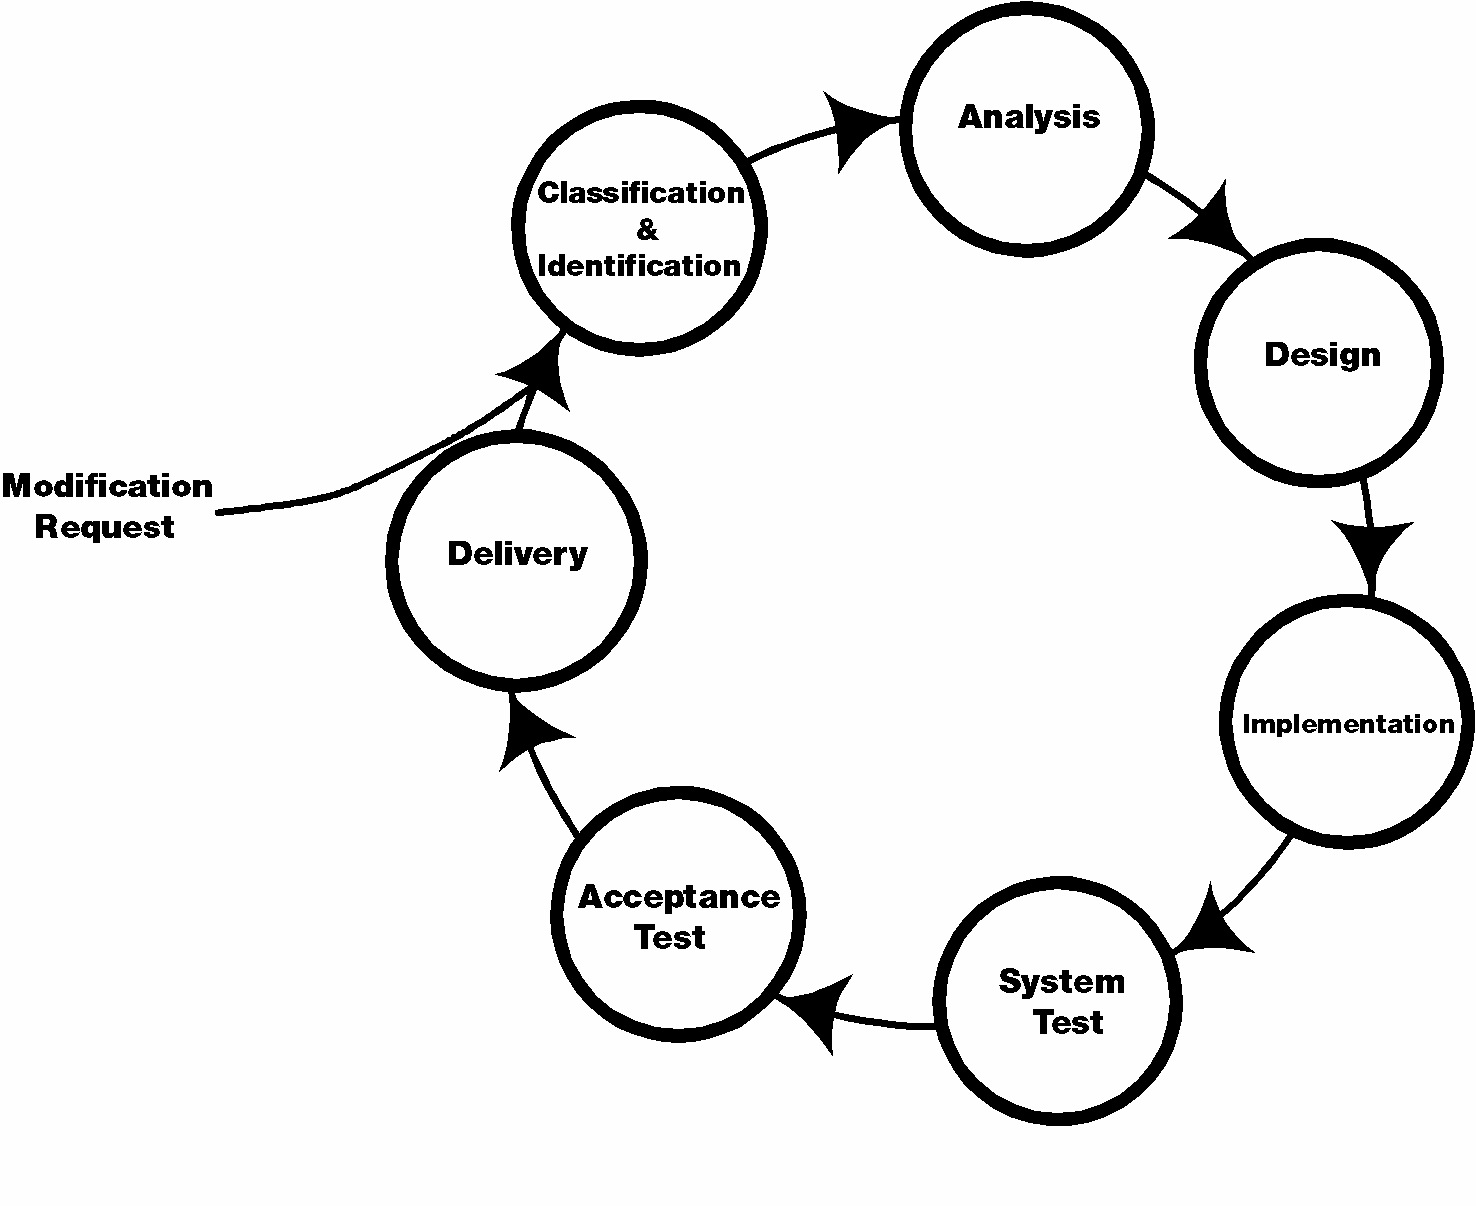
\includegraphics[width=0.7\linewidth]
	{./chapter-manutencao-software-visao-geral/img/ieee-1219-98-processo-manutencao.png}
	\caption{IEEE 1219 -~Processo de Manutenção de Software}\label{fig:ieee-1219-processo-man-software}
\end{figure}

De maneira relacionada, na ISO/IEC 14764 as atividades que compõe o processo são
similares aquelas propostas na IEEE-~1219, exceto pelo fato que elas são
agregadas de uma forma diferente. O processo descrito na ISO/IEC~14764 são
exibidas na Figura~\ref{fig:ieee-14764-processo-manutencao}

\begin{figure}[htpb] \centering
	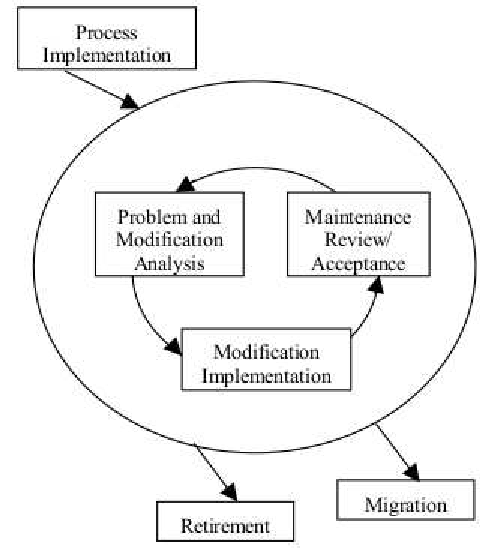
\includegraphics[width=0.7\linewidth]
{chapter-manutencao-software-visao-geral/img/ieee-14764-processo-manutencao.pdf}
	\caption{ISO/IEC~14764 Processo de Manutenção de Software}
\label{fig:ieee-14764-processo-manutencao} \end{figure}

As atividades de manutenção propostas na ISO/IEC 14764 são detalhadas em tarefas
conforme apresentadas a seguir:

\begin{itemize}
   	\item Implementação do Processo
   	\item Análise e Modificação do
		Problema
	\item Aceitação e Revisão da Manutenção
   	\item Migração
   	\item Aposentadoria do Software
\end{itemize}

É possível notar que algumas atividades realizadas durante a manutenção de
software são similares à outras presentes no desenvolvimento de software, como
por exemplo, análise de desempenho, codificação, teste e documentação. Outra
atividade comum à manter e desenvolver software é o gerenciamento dos
requisitos. Nas duas situações os profissionais responsáveis por controlar os
requisitos devem atualizar a do\-cu\-men\-ta\-ção  por conta de alterações
ocorridas no código fonte. Por outro lado certas atividades estão vinculadas
apenas ao contexto da manutenção de software. O Corpo de Conhecimento em
Engenharia de Software~\cite{4425813} destaca algumas delas:

\todobegin{Faltava referência sobre as atividades que seriam únicas ao processo
	de manutenção. Havida duvidas sobre se as atividades: Suporte ao Usuário,
	Suporte ao Uso de Software e Acordo de Nível de Serviço}
\begin{description}
	\item[Compreensão do programa:] atividades necessárias para obter um
		conhecimento geral do que um produto de software faz e como as partes
		funcionam em conjunto;
	\item[Transição:] uma sequência controlada e coordenada de atividades onde o
		software é transferido progressivamente do desenvolvedor para o
		mantenedor;
	\item[Aceitação/rejeição de Requisições de Mudança:] as modificações
		que ultrapassem determinado limiar de tamanho, esforço ou complexidade
		podem ser rejeitadas pelos mantenedores e redirecionadas para um
		desenvolvedor;
	\item[Suporte ao usuário:] uma função de suporte para o usuário final que
		aciona a priorização ou avaliação de esforço das Requisições
		de Mudança;
	\item[Análise de impacto:] uma técnica para identificar os módulos que
		possivelmente pode ser afetado por determinada mudança solicitada;
	\item[Contratos de Acordo de Nível de Serviço (Service Level Agreements
		\@-\@ SLA):] acordos contratuais que descrevem os serviços a serem
		realizados pela equipe de manutenção e os objetivos de qualidade do
		produto de software.
\end{description}
\todoend

\subsubsection{Manutenção de Software na Perspectiva dos Agilistas}
\label{sub:manutenção_de_software_com_método_dos_agilistas}

Grande parte da literatura em Manutenção de Software trata de técnicas e
metodologias tradicionais da Engenharia de Software. Todavia, verifica-se uma
tendência que os departamentos dedicados à manutenção de software se mostrem
interessados nas metodologias dos agilistas e que tenham vontade de
experimentá-las em suas atividades~\cite{Heeager2015}.

No momento da elaboração desta dissertação boa parte dos textos em Engenharia de
Software tratarem desenvolvimento e manutenção como atividades com natureza
distintas, esta última pode adaptar características da primeira visando a
melhoria do seu desempenho. Dentre as práticas propostas pelos agilistas
passíveis de serem utilizadas em tarefas de manutenção é possível citar o
desenvolvimento iterativo, maior envolvimento do cliente, comunicação face a
face, testes frequentes, dentre outras.

Alguns resultados demonstram certa dificuldade para implantação da metodologia
dos agilista na manutenção de software~\cite{1402140}. Um dos possíveis
problemas é a necessidade de adequação das práticas da organização de modo que a
se adequar as necessidades do time de desenvolvimento.  Estudos apresentam
resultados relativos à melhorias no aprendizado e produtividade da equipe
mediante o aumento da moral, encorajamento e confiança entre os desenvolvedores,
o que propicia uma alta motivação durante o processo de manutenção de
software~\cite{Choudhari:2014:EIM:2557833.2557845}.

\todobegin{Conforme sugerido vou ``deslocada'' a discussão sobre os papéis
	dentro da manutenção de software. O testo foi revisado e para deixar mais
	claro foi utilizada diagrama de caso de uso.}

\subsection{Papéis na Manutenção de Software}
\label{subsec:man_visao_geral_papeis_na_manutencao_de_software}

As ações que alteram o estado de uma RM são realizadas por diversas pessoas
envolvidas no processo de manutenção de software. Neste processo cada integrante
da equipe de manutenção pode desempenhar um ou mais papéis. Os nomes e as
atividades desenvolvidas por cada papel pode variar de um projeto para outro,
contudo, é possível determinar uma classificação que agregue um ponto comum
destes diferentes papéis. Nesta dissertação, utilizamos a classificação proposta
por Polo e outros~\cite{Polo1999} cujo objetivo é definir uma estrutura da
equipe de manutenção de software mediante a clara identificação das tarefas que
cada membro deve executar. Os papéis propostos no estudo é produto da aplicação
da metodologia MANTEMA~\cite{756695} em projetos de software bancários
espanhóis, em especial aqueles em que a área de manutenção foi terceirizada
(outsourcing). Os autores reforçam que apesar da taxonomia de papéis ter sido
criada em um contexto específico, ela pode ser adequada para aplicação em outras
situações.

No escopo deste trabalho removemos os papéis que segundo o nosso entendimento
estão mais vinculados a um contexto de manutenção terceirizada (outsourcing).
Além disso, dividimos o papel ``time de manutenção' (maintenance team) em
\textit{Desenvolvedor e Analista de Qualidade} por entendermos que são papéis
comuns a muito dos processos de manutenção existentes. Os papéis que compõe a
taxonomia proposta estão descritos a seguir:

\paragraph{Usuário Afetado:}
Indivíduo que utiliza o sistema ou sistemas que correspondente à RM que será
relatada. O defeito, a melhoria ou evolução no software, representada pela RM,
estão relacionadas com os desejos e necessidades deste papel.

\paragraph{Reportador:}
Responsável por registrar a Requisição de Mudança na FGRM\@. Geralmente,
qualquer pessoa envolvida no processo de manutenção de software pode relatar uma
RM. Neste sentido, as atividades relacionadas com o papel de Reportador podem
estar vinculados com outras contidas nesta classificação. A
Figura~\ref{fig:diagrama-caso-uso-reportador} apresenta esta situação através de
um diagrama de caso de uso, onde o \textit{Reportador} pode ser um usuário do
sistema ou mesmo um membro da equipe de manutenção.

\begin{figure}[htpb]
	\centering
	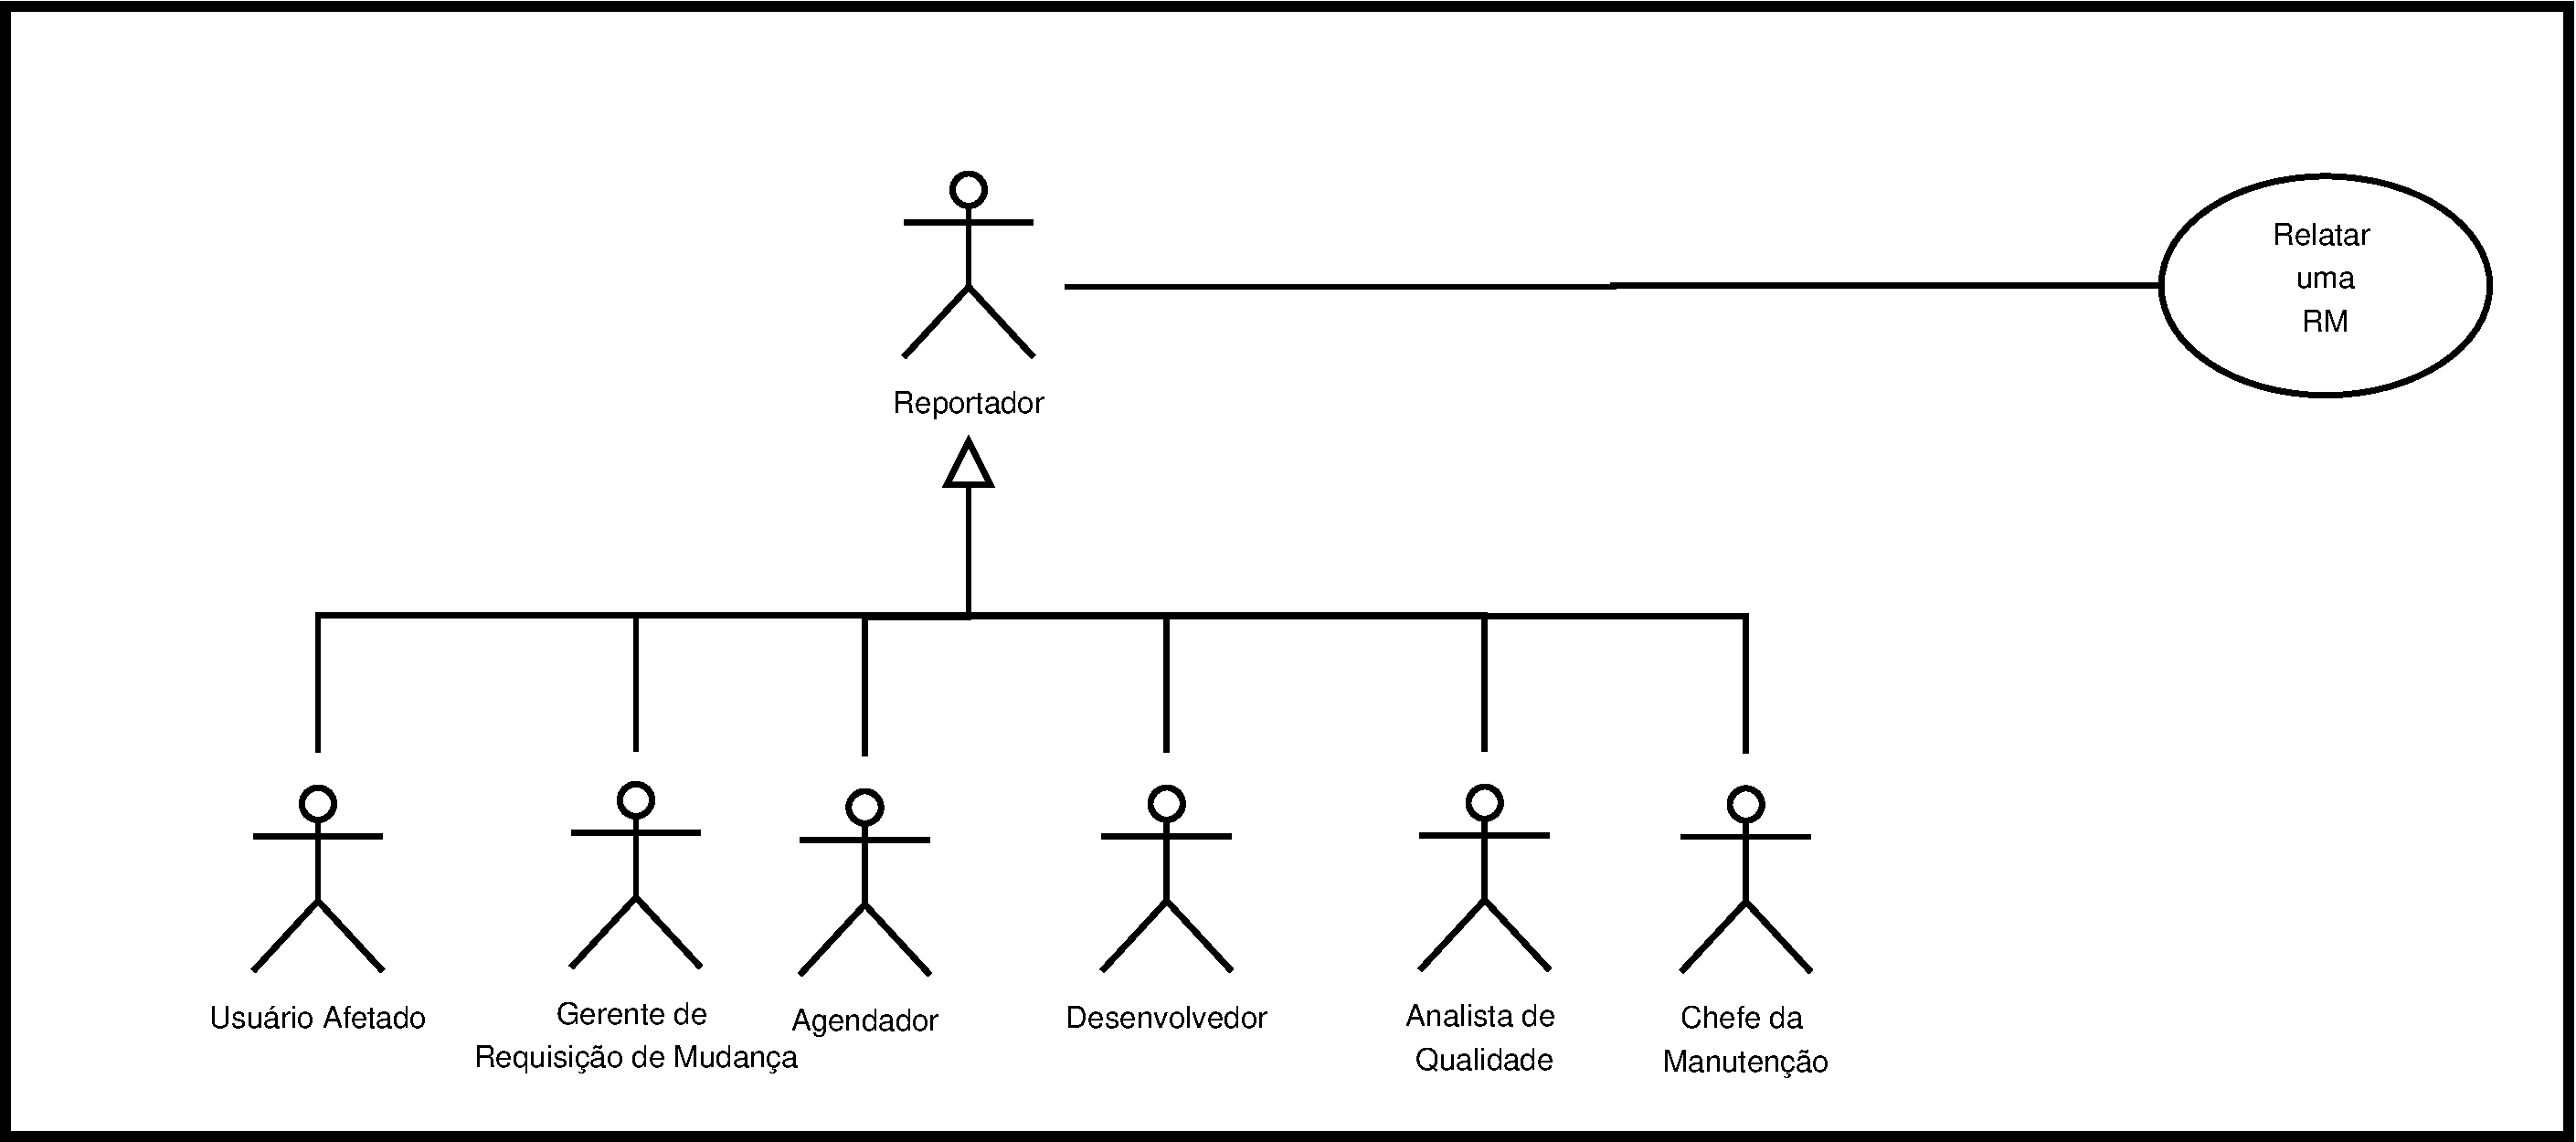
\includegraphics[width=0.8\linewidth]{./chapter-manutencao-software-visao-geral/img/diagrama-caso-uso-reportador.pdf}
	\caption{Diagrama de caso de uso do papel Reportador}
	\label{fig:diagrama-caso-uso-reportador}
\end{figure}

\paragraph{Gerente de Requisição de Mudança (Maintenance-request manager):}
Res\-pon\-sá\-vel por decidir se uma Requisição de Mudança será aceita ou
rejeitada e qual tipo de manutenção deverá ser aplicada. Posteriormente cabe a
ele/ela encaminhar a RM para o Agente de Triagem.

\paragraph{Agente de Triagem (Scheduler)}:
Deve planejar a fila de Requisições de Mudança aceitas. Também estão no rol de
responsabilidades deste papel a atribuição das RM's para o desenvolver mais
apto.

\paragraph{Desenvolvedor:}
Responsável por realizar as ações que irão solucionar a Requisição de Mudança.

\paragraph{Analista de Qualidade:}
Responsável por avaliar se uma Requisição de Mudança que foi solucionada por um
Desenvolvedor afim de verificar se a RM foi resolvida de forma correta.

\paragraph{Chefe da Manutenção (Head of	Maintenance):}
Tem por responsabilidade definir os padrões e procedimentos que compõe o
processo de manutenção que será utilizado.

Apesar da classificação de papéis utilizada derivar de um contexto de manutenção
de software específico (setor bancário e empresas com a área de manutenção
terceirizada), ela é capaz de acoplar com outros tipos de processo de manutenção
de software, como aquele proposto por Ihara e outros
\cite{Ihara:2009:AMI:1595808.1595833}. Naquele estudo foi criada uma
representação de um processo de modificação de bugs tomando como base as
diversas situações que um bug possui em uma FGRM no contexto de projetos de
código aberto. O processo resultante é facilmente acoplável com a classificação
utilizada em nosso estudo.

Cabe ressaltar que está fora do escopo deste estudo elaborar uma taxonomia dos
papeis envolvidos na Manutenção de Software em função de supormos que isto
corresponde a um esforço bem extenso. Nossa ação é identificar se existem papeis
e quais são eles, sem com isso, envolver em uma consolidação definitiva.
\todoend

\subsection{Requisição de Mudança}
\label{sec:requisicao_de_mudanca}

\subsubsection{Tipos de Requisições de Mudança}
\label{subsec:tipos_de_requisicoes_mudanca}

As manutenções em software podem ser divididas em \textit{Corretiva, Adaptativa,
	Perfectiva e Preventiva}~\cite{Lientz:1980:SMM:601062,159342}.  A Manutenção
Corretiva lida com a reparação de falhas encontradas. A Adaptativa tem o foco na
adequação do software devido à mudanças ocorridas no ambiente em que ele está
inserido. A Perfectiva trabalha para detectar e corrigir falhas latentes. A
Preventiva preocupa com atividades que possibilitem aumento da manutenibilidade
do sistema.  A ISO 14764~\cite{1703974} propõe a divisão da tarefa de
manutenção nos quatro tipos descritos anteriormente e propõe que exista um
elemento comum denominado Requisição de Mudança (RM) que representa as
características comuns a todas aqueles tipos de manutenção. A
Figura~\ref{fig:modification-request} exibe a classificação das RM's conforme
discutido pela ISO\@.

\begin{figure}[hbtp] \centering 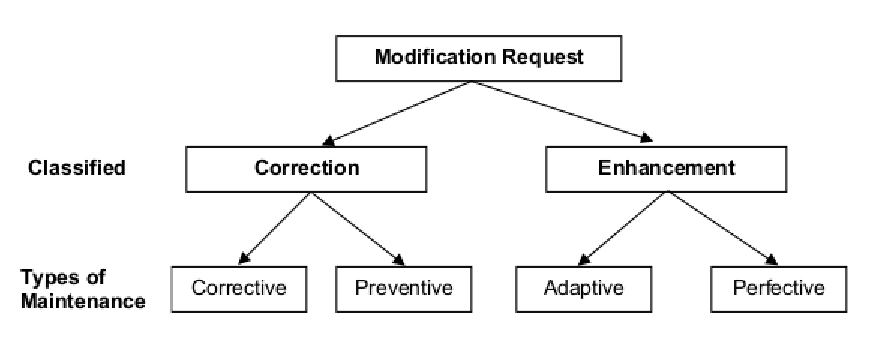
\includegraphics[width=.75\textwidth]
	{./chapter-intro/img/modification_request.eps} \caption{Tipos de manutenção
		segundo a norma ISO/IEC 14764. Extraído de~\cite{1703974}}
\label{fig:modification-request} \end{figure}

A ISO/IEC 14764 classifica as manutenções adaptativas e perfectivas como
me\-lho\-ri\-as e agrupa as manutenções corretivas e preventivas em uma única
categoria de correção, conforme exibido na
Tabela~\ref{tab:categorias_requisicao_mudanca}. A manutenção preventiva é
frequentemente realizada em produtos de software onde atributos de segurança são
mais críticos.

\begin{table}[htpb] \centering 	\begin{tabular}{l|l|l|} \cline{2-3} &
		\textbf{Correção} & \textbf{Melhoria} \\ \hline
		\multicolumn{1}{|l|}{\textbf{Pró-ativa}} & Preventiva & Perfectiva \\
		\hline \multicolumn{1}{|l|}{\textbf{Reativa}} & Corretiva & Adaptativa
		\\ \hline \end{tabular}\caption{Categorias da Requisição de Mudanças.
		Adaptado de
		SWEBOK~\cite{4425813}}\label{tab:categorias_requisicao_mudanca}
\end{table}

\todobegin{Incluída discussão sobre os atributos e classificação de uma RM.}

Alguns pesquisadores e profissionais entendem a manutenção preventiva como um
subconjunto da perfectiva~\cite{tripathy2014software}.  Segundo Tripathy \& Naik
uma Requisição de Mudança (RM) é o veículo para registrar a informação sobre o
defeito, evolução ou melhoria de um sistema. Com base no que é discutido pelos
autores construímos o modelo conceitual exibido na
Figura~\ref{fig:diagrama-classe-requisicao-mudancas}. No modelo, uma RM é
especializada como um \textit{Pedido de Correção} de determinada falha ou como
um \textit{Pedido de Melhoria} que pode estar relacionado com o aprimoramento de
funcionalidades ou com a melhoria da qualidade do sistema. Alguns autores
utilizam os termos \textit{relato de defeito ou relato de melhoria} como
sinônimos para a RM, contudo, conforme discutido posteriormente, o relato, que é
o texto livre que descreve a RM, é um dos atributos que a compõe (vide
Figura~\ref{fig:diagrama-classe-atributos-requisicao-mudancas}).

\todobegin{Incluída uma imagem para representar que a Requisição de Mudanças
	representam um elemento comum de relatos de defeitos, evolução ou melhoria
	de um sistema}
\begin{figure}[htpb]
	\centering
	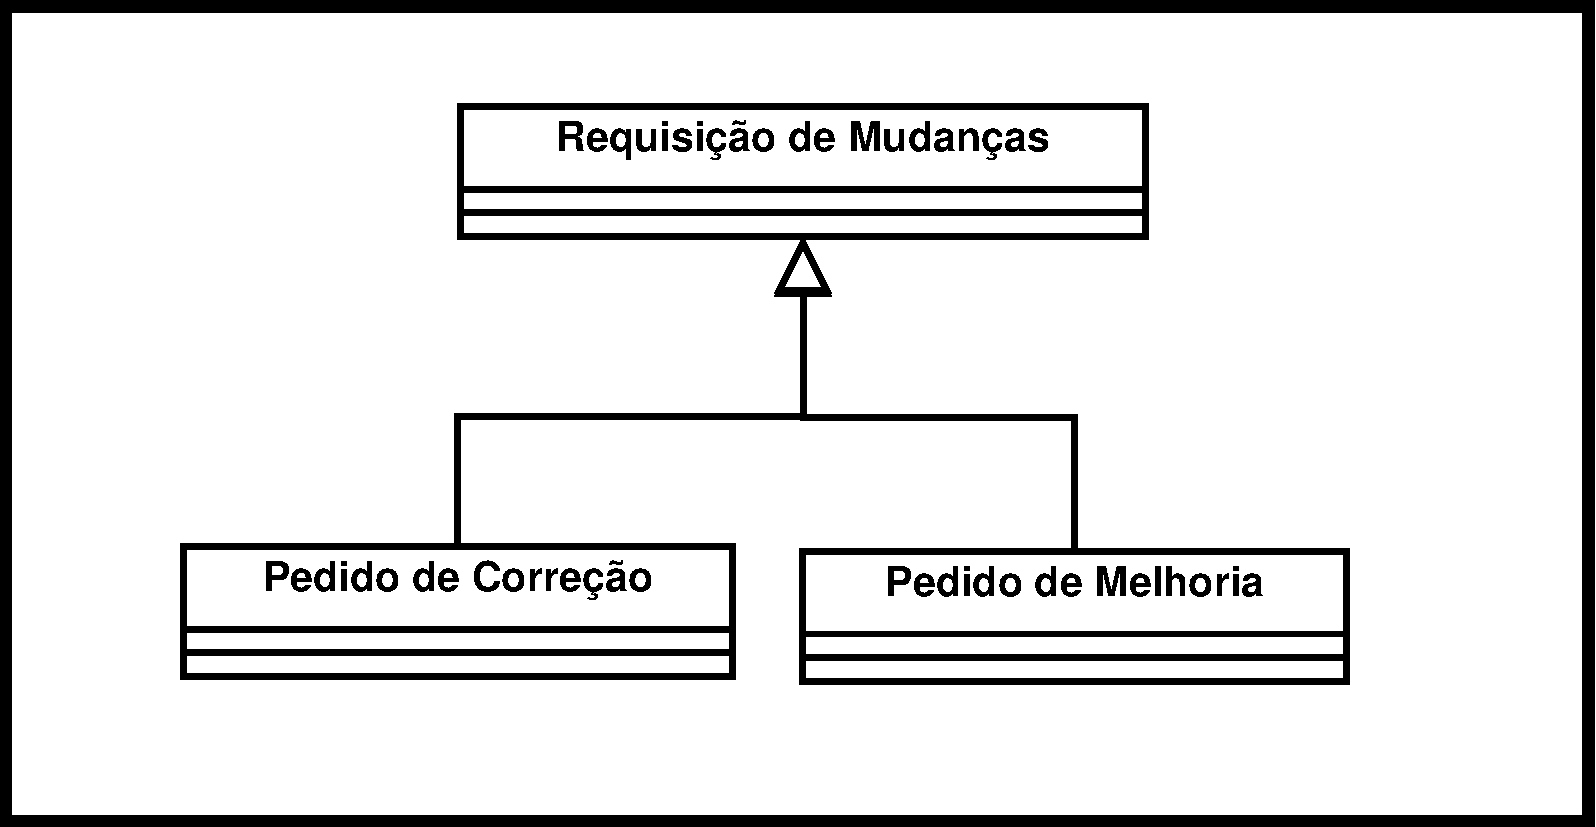
\includegraphics[width=0.8\linewidth]{./chapter-manutencao-software-visao-geral/img/diagrama-classe-conceitual-requisicao-mudancas.pdf}
	\caption{Modelo conceitual de uma Requisição de Mudanças}
	\label{fig:diagrama-classe-requisicao-mudancas}
\end{figure}
\todoend

As principais informações contidas em uma RM podem ser visualizadas no modelo
exibido na Figura~\ref{fig:diagrama-classe-atributos-requisicao-mudancas}. O
modelo é uma adaptação daquele proposto no trabalho de Singh \&
Chaturvedi~\cite{singh2011bug} onde é descrito um processo genérico de como uma
RM é relatada.

\begin{figure}[htpb]
	\centering
	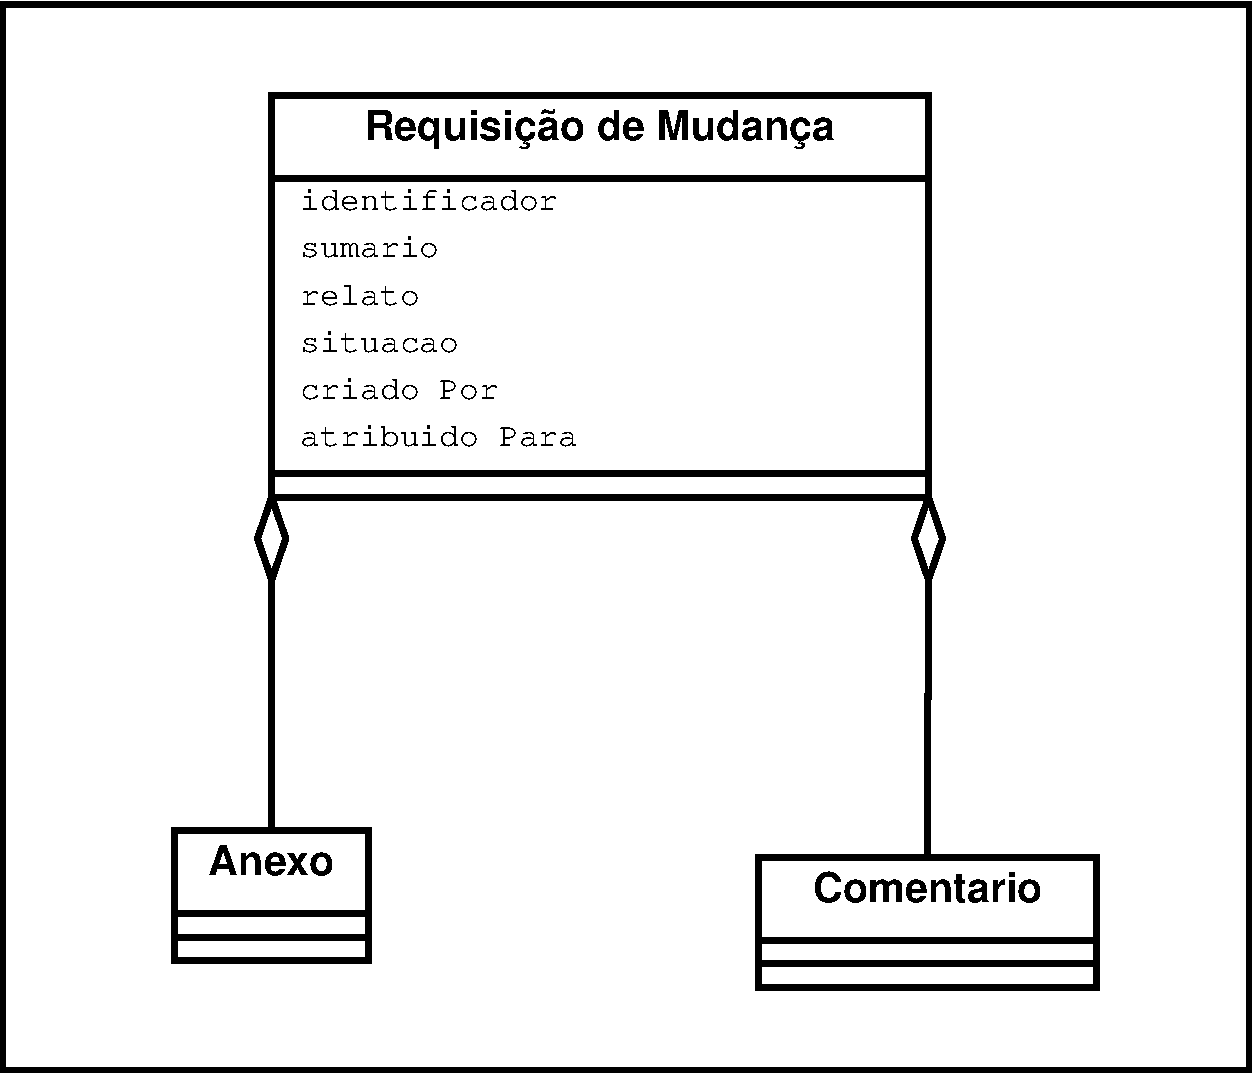
\includegraphics[width=0.8\linewidth]{./chapter-manutencao-software-visao-geral/img/diagrama-classe-atributos-requisicao-mudancas.pdf}
	\caption{Informações que compõem uma RM}
	\label{fig:diagrama-classe-atributos-requisicao-mudancas}
\end{figure}

Os principais conceitos envolvidos no modelo estão descritos a seguir:

\begin{description}
	\item [Identificador] Sequência de caracteres,  geralmente numérica,  que
		permite distinguir de maneira única uma RM.
	\item [Sumário] Um título ou resumo da RM.
	\item [Relato] Descrição detalhada da RM incluindo o que, onde, por que,
		como e quando a situação relatada na RM ocorreu. A mensagem que aparece
		durante a operação do sistema pode ser incluída, bem como a entrada
		inserida e/ou a saída esperada.
	\item [Situação] A situação atual de uma RM\@. Representa os diversos
		estados que uma RM possui em seu ciclo de vida. Nesta dissertação
		discutimos brevemente o ciclo de vida de uma RM na Subseção
		~\ref{sub:fluxo_de_trabalho_requisicao_mudanca}.
	\item [Criado Por] Nome da pessoa ou um identificador já registrado no
		sistema de quem criou a RM\@.
	\item [Atribuido Para] A RM pode ser atribuída a uma pessoa específica caso
		ela seja capaz de resolvê-la, caso contrário, a RM será atribuída para
		alguém que possui o papel de definir o desenvolvedor mais apto para
		solucionar aquela RM. Neste estudo, o membro de uma equipe de manutnçaõ
		com festa função é denominado \textit{Agente de Triagem}.
	\item [Anexo] Refere-se a informação que não estejam em formato de texto e
		que podem ser incluídas na RM como casos de teste, capturas de tela,
		cadeia de registros de ativação (stack trace), dentre outros.
	\item [Comentário] Registra o histórico de discussões realizadas durante o
		processo de resolução da RM\@.
\end{description}

\todobegin{Incluída uma breve discussão sobre os motivos que determinados
	atributos foram modelados como agregação e outros não.}

Conforme pode ser observado na Figura
~\ref{fig:diagrama-classe-atributos-requisicao-mudancas} os atributos
\textit{Comentário} e \textit{Anexo} foram modelados com agregação, dando aos
mesmos um caráter multivalorados. Esta escolha foi intencional de modo a
salientar que determinada instância de uma RM pode conter diversos anexos ou
comentários. No caso dos comentários esta característica é ainda mais relevante
tendo em vista que o conjunto de comentários realizados durante do processo de
solução de uma RM possui informações relevantes para o software sendo mantido,
já que, por exemplo, pode ser utilizada para solucionar futuras RM's. 

Os atributos que compõem uma RM pode variar dependendo da ferramenta que a
gerencia, o projeto ao qual esteja vinculada, dentre outros fatores. Tais
campos, denominados de pré-definidos, fornecem uma variedade de metadados
descritivos tais como \textit{importância, prioridade, gravidade, componente, e
	produto}~\cite{zhang2016literature}. A Figura~\ref{fig:rm-exemplo} exibe um
exemplo representativo de uma RM contendo todos os elementos básicos descritos
no modelo proposto na
Figura~\ref{fig:diagrama-classe-atributos-requisicao-mudancas} tais como
identificador, sumário, relato e outros.

\begin{figure}[htpb]
	\centering
	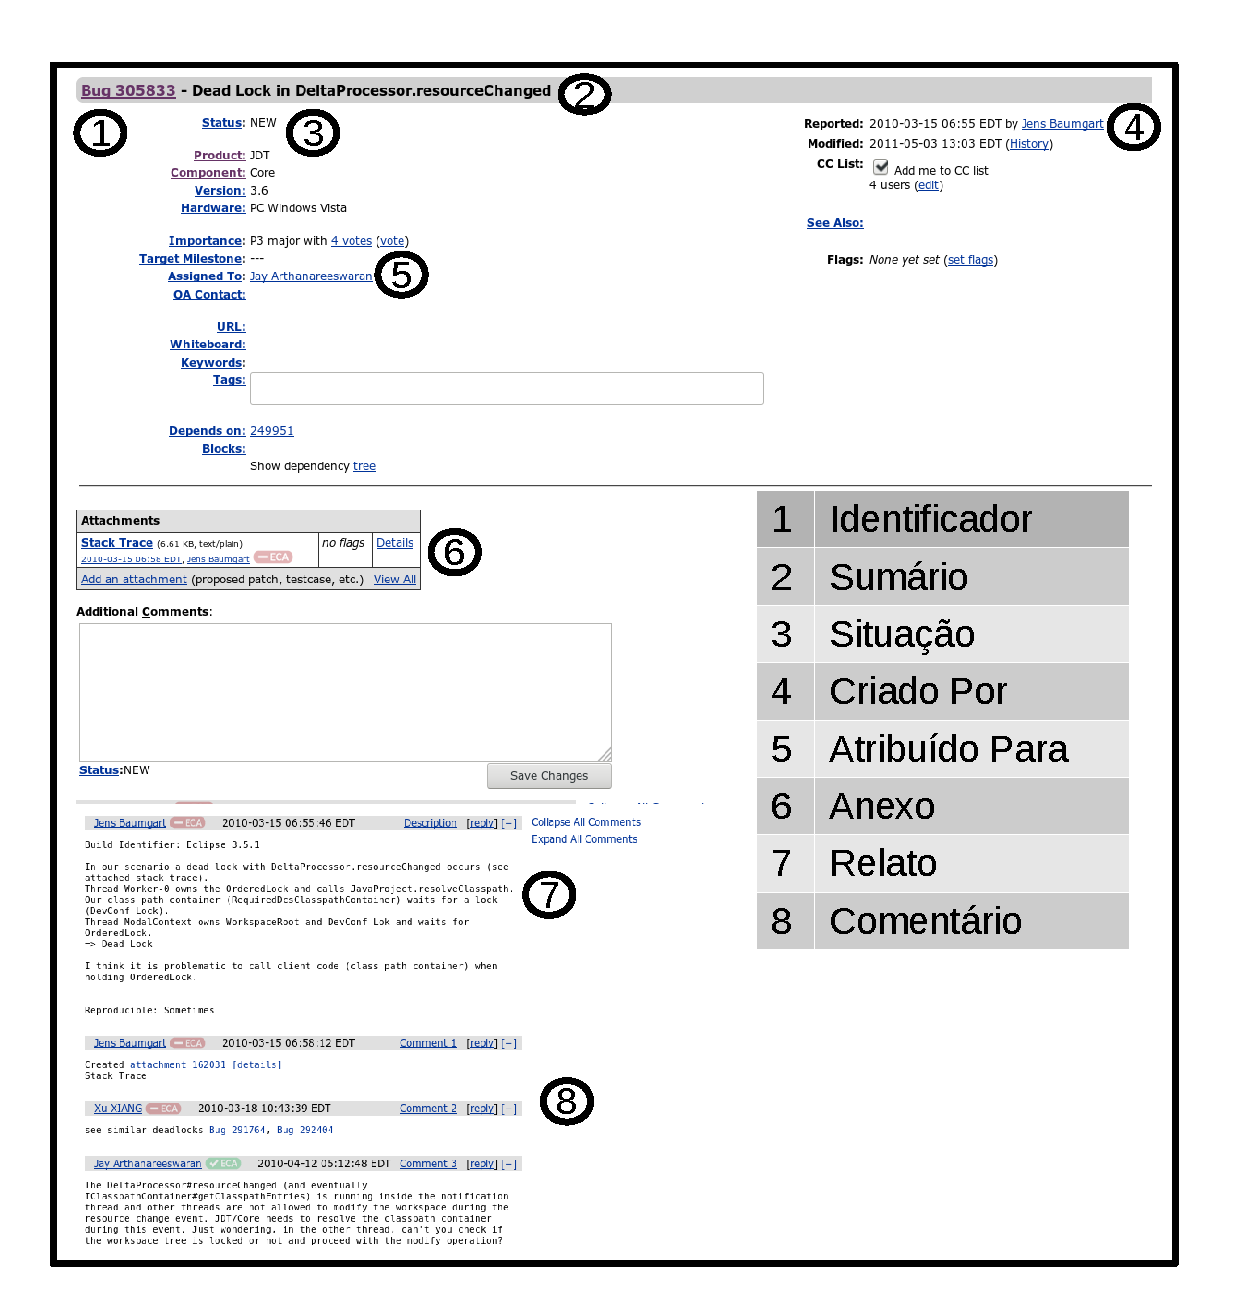
\includegraphics[width=0.8\linewidth]{./chapter-manutencao-software-visao-geral/img/rm-exemplo.pdf}
	\caption{Um exemplo de uma RM do Projeto Eclipse}
	\label{fig:rm-exemplo}
\end{figure}
\todoend

\todobegin{Rodolfo, você acha que faz sentido o parágrafo a seguir?}
Em síntese, apesar das diferentes nomenclaturas existentes na literatura
(demanda, bug, defeito, bilhete, tíquete, requisição de modificação, relato de
problema) uma Requisição de Mudança representa o relato, independente de sua
estrutura, que visa gerar a manutenção ou evolução do software. Nesta
dissertação estas diferentes nomenclaturas serão utilizados de forma
intercambiáveis.

\subsubsection{Ciclo de Vida de uma Requisição de Mudança}
\label{sub:fluxo_de_trabalho_requisicao_mudanca}
\todobegin{Incluída uma discussão sobre os diversos ``estados'' que um
	determinada RM pode ter. Os conceitos foram apoiados no livro Software
	Evolution and Maintenance de Priyadarshi e Kshirasagar}

Uma RM descreve os desejos e necessidades dos usuário de como um sistema deve
operar. Durante o processo de relatar uma RM, dois fatores devem ser levados em
conta~\cite{tripathy2014software}:

\begin{itemize}
	\item \textit{Corretude da RM:} uma RM deve ser descrita de forma não
		ambígua tal que seja fácil revisá-la afim de determinar sua corretude. O
		``formulário'', que são os campos que devem ser preenchidos na RM, são a
		chave para efetiva interação entre a organização que desenvolver o
		software e os seus usuários. O formulário, neste sentido, documenta
		informações essenciais sobre mudanças no software, hardware e
		documentação.
   \item \textit{Comunicação clara das RM's com as partes
		   interessadas:\footnote{Na
			   Seção~\ref{subsec:man_visao_geral_papeis_na_manutencao_de_software}
			   discutiremos em maior detalhe as diferentes partes interessadas
			   no contexto da manutenção de software.}} as RM'S necessitam ser
	   claramente comunicadas para que todas as parte as interessadas, incluindo
	   os mantenedores, interpretem de maneira similar o que foi solicitado. O
	   resultado de avaliar de maneira distinta uma RM pode ser
	   contra-produtivo: \textit{(i)} a equipe que realiza mudanças no sistema e
	   a equipe que executa testes podem ter  visões contraditórias sobre a
	   qualidade do software; \textit{(ii)} O sistema alterado pode não atender
	   às necessidades e desejos dos usuários finais.
\end{itemize}

No caminho entre o usuário que a relata e os desenvolvedores que a soluciona,
uma RM pode estar em diferentes estágios. O ciclo de vida de uma RM pode ser
ilustrado como diagrama de estados conforme ilustrado na
Figura~\ref{fig:diagrama-estado-rm}. Naquele modelo uma RM inicia com o estado
\textit{Submetida (Submit)} e vai sendo modificada até alcançar o estado
\textit{Fechada (Closed)} onde ela foi finalmente solucionada. Neste caminho,
entre os diversos estágios intermediários, o conjunto de fatores que resultou na
necessidade de relatar uma RM pode não mais existir. Neste caso, ela é alterada
para o estado \textit{Rejeitada (Decline)}.

\begin{figure}[htpb]
	\centering
	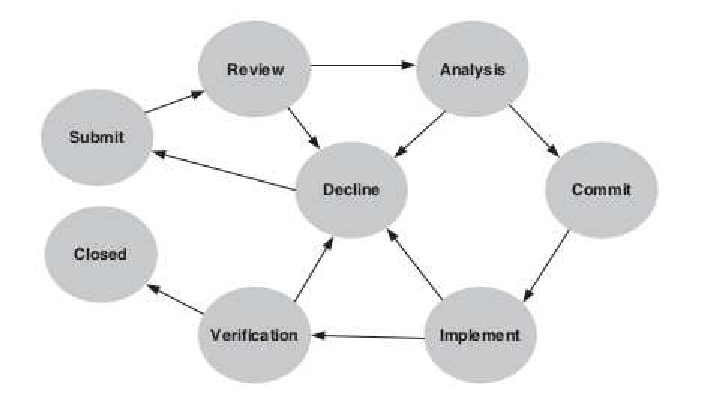
\includegraphics[width=0.8\linewidth]{./chapter-manutencao-software-visao-geral/img/diagrama-estado-rm.pdf}
	\caption{Diagrama de estados de uma RM\@. Extraído
		de~\cite{tripathy2014software}}
\label{fig:diagrama-estado-rm}
\end{figure}

O modelo mostra a evolução de uma RM mediante os seguintes estados:
\textit{Submetida (Submit), Em Revisão (Review), Em análise (Analysis), Commit
	(Comprometida), Em Implementação (Implement), Em Verificação (Verification) e
	Fechada (Closed)}~\cite{tripathy2014software}. Uma determinada RM também
pode ser rejeitada o que a leva para o estado de mesmo nome
(\textit{Rejeitada - Decline}).
Por diversas razões a situação de uma RM pode ser alterada para
\textit{Recusada} a partir dos outros estados. Um exemplo desta situação ocorre
quando um  usuário conclui que modificações descritas na RM não fazem mais
sentido.

A seguir apresentamos as características de cada um dos estados que compõem o
ciclo de vida de uma RM\@. Para cada estado pode haver mais de um papel
responsável pelas ações que são executadas. Também pode ocorre que uma mesma
pessoa desempenhe diferentes papéis neste processo. Uma discussão sobre este
papeis pode ser encontrada na
Subseção~\ref{subsec:man_visao_geral_papeis_na_manutencao_de_software}.

\paragraph{Submetida (Submit).}
\label{par:submetida)}

Este é o estado inicial de uma RM recentemente envida. Geralmente, são os
usuários do sistema a fonte primária das RM nesta situação. Com base no nível de
prioridade de uma RM, ela é movida de \textit{Submetida} para \textit{Em
	Revisão}. Normalmente cabe ao \textit{Gerente de Requisição de Mudança} a
responsabilidade desta manipulação inicial das RM's. Neste instante ele se torna
o ``dono'' da RM.

\paragraph{Em Revisão (Review).}
\label{par:em_revisao}
Normalmente, cabe ao \textit{Gerente de Requisição de Mudanças} manipular as
RM's no estado \textit{Em Revisão} através das seguintes atividades:

\begin{itemize}
	\item Verificar se a RM submetida recentemente é idêntica de outra já
		existente. Se a RM é identificada como duplicada o estado da mesma é
		alterado para \textit{Rejeitada}. Neste casos, uma breve explicação e
		algum tipo de ligação para a original são inseridos nos comentários da
		RM.
	\item Aceitar o nível de prioridade atribuído para a RM ou alterá-lo.
	\item Determinar o nível de severidade da RM: normal ou crítico.
	\item Caso por alguma razão as análises descritas anteriormente não possam
		ser re\-a\-li\-za\-das, a RM é movida para o estado em \textit{Em análise}.
\end{itemize}

\paragraph{Em Análise (Analysis).}
\label{par:em_analise}
Neste estágio uma análise de impacto é conduzida para entender a RM e estimar o
tempo necessário para implementá-la. Após esta análise, caso se decida que não é
possível ou desejável atender a RM, então \textit{Rejeitada} se torna o próximo
estágio da RM. Caso contrário a RM é movida para estado \textit{Comprometida
	(Commit)}. No  \textit{Em Análise} o ``dono'' da RM é denominado
\textit{Agente de Triagem}.

\paragraph{Comprometida (Commit).}
\label{par:commit}

A RM continua ``parada'' no estado \textit{Comprometida} antes que as
modificações solicitadas possam ser implementadas e estejam disponíveis em uma
próxima versão do produto. Neste estado a RM está a cargo do \textit{Gerente de
	Requisição de Mudança}. Algumas RM's podem ser incluídas em futuras versões
do sistema após acordo com as demais partes interessadas. Após
\textit{Comprometida} com determinado lançamento, a RM é movida para o estado
\textit{Em Implementação} para que o respectivo desenvolvimento e testes sejam
realizados.

\paragraph{Em Implementação (Implement).}
\label{par:em_implementacao}

No estágio de \textit{Em Implementação} diferentes cenários podem ocorrer:

\begin{itemize}
	\item A RM pode ser rejeitada caso sua implementação não seja factível.
	\item Caso a RM seja possível de implementar os desenvolvedores realizam a
		codificação e os testes. Após finalizada a codificação a RM é movida de
		\textit{Em Implementação} para \textit{Em verificação}.
\end{itemize}

\paragraph{Em Verificação (Verification).}
\label{par:em_verificacao}

No estão de verificação as atividades são controladas pela equipe de testes.
Para atribuir um veredito, a verificação pode ser realizada por um ou mais
métodos: demostração, análise, inspeção ou teste. No primeiro caso, o software é
executado com um conjunto de teste. A inspeção significa revisar o código em
busca de defeitos. No caso da análise, o processo consiste em demonstrar que o
sistema está em operação.

\paragraph{Fechada (Closed).}
\label{par:fechada}

Após a verificação de que a RM foi incorporada com sucesso ao software, a RM é
movida de \textit{Em verificação} para o estado \textit{Fechada}. Esta ação é
realizada pelo \textit{Analista de Qualidade} que o proprietário da RM durante o
estado de \textit{Em Verificação}.

\paragraph{Rejeitada (Decline).}
\label{par:rejeitada}

Conforme discutido uma RM pode ser rejeitada. Nestas situações a RM é movida
para um estado de mesmo nome. Dentre os diversos motivos que levam uma RM deixar
de ser feita podemos destacar: a RM deixar de produzir relevante impacto no
sistema; não é possível tecnicamente realizar o que foi solicitado na RM; a
equipe de qualidade conclui que as mudanças realizadas no software pela RM não
podem ser satisfatoriamente verificadas.
\todoend

\todobegin{Incluída a visão do processo de ciclo de vida de uma RM em projetos
	de código aberto.}

O modelo de ciclo de vida discutido por Tripathy \& Naik possui um foco na
industria de software, especialmente em organizações que possuem uma área
exclusivamente dedicada à manutenção de software. Em outros contextos, como por
exemplo em projetos de software de código aberto, o processo de modificação dos
estados de uma RM é um pouco diferente.

No trabalho de Ihara e outros~\cite{ihara2009analysis}, foi conduzido um estudo
de caso nos projetos de código aberto Firefox e Apache em que um dos resultados
foi um digrama de estados que representa o processo de modificação de uma RM
utilizando uma FGRM. Este diagrama é representado na
Figura~\ref{fig:diagrama-estado-rm-codigo-aberto}.

\begin{figure}[htpb]
	\centering
	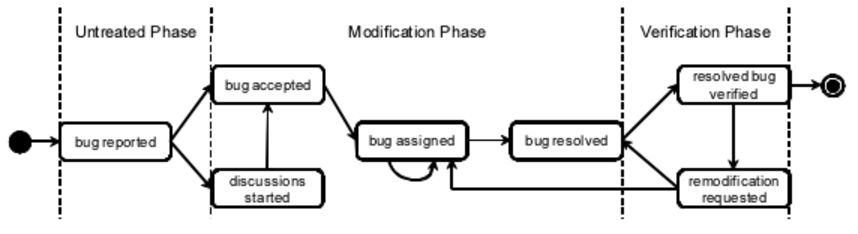
\includegraphics[width=0.8\linewidth]{./chapter-manutencao-software-visao-geral/img/diagrama-estado-rm-codigo-aberto.pdf}
	\caption{Um processo de modificação de uma RM utilizando uma FGRM. Extraído
	de~\cite{ihara2009analysis}}
	\label{fig:diagrama-estado-rm-codigo-aberto}
\end{figure}

Os autores ponderam que apesar do processo de modificação de uma RM pode alterar
levemente de uma FGRM para outra, o diagrama apresentado na
Figura~\ref{fig:diagrama-estado-rm-codigo-aberto} é capaz de representar de forma
substancial o processo de transição de uma RM. O processo é composto de três
diferentes fase: \textit{não tratada (untreated) , modificação (modification) e
verificação (verification)}.

A fase \textit{não tratada} foca em um subprocesso onde as RM's são relatadas em
uma FGRM, todavia não foi aceito ou atribuída a ninguém. A fase de
\textit{modificação} é um subprocesso onde as RM's são efetivamente modificadas.
Nesta fase uma RM é aceita e posteriormente atribuída a algum desenvolvedor.  A
fase de \textit{verificação} é o subprocesso onde membros com a responsabilidade
de garantia da qualidade verificam quais RM's modificadas foram corretamente
resolvidas. Caso uma RM modificada por um desenvolver não seja verificada, ela
poderia não ser reconhecida como fechada (closed).

É possível acoplar o modelo proposto por Tripathy \&
Naik~\cite{tripathy2014software} naquele descrito por Ihara e
outros~\cite{ihara2009analysis}, especialmente por conta do segundo ser mais
genérico.  Neste dissertação utilizamos de forma geral o modelo contido no
trabalho de Ihara e outros. Nos casos em que houver necessidade de um maior
detalhamento do ciclo de vida de uma RM, a discussão tomará como base o modelo
de Tripathy \& Naik.
\todoend

\todobegin{Incluída seção sobre conceituamos os problemas relacionados à gestão
da RM's.}

\subsubsection{Problemas Relacionadas à Gestão da RM}
\label{ssub:problemas_relacionadas_rm}

A literatura discute e apresenta diversos problemas relacionadas à gestão das
RM's:

\paragraph{Identificação de RM Duplicadas} O processo de identificação de RM's
Duplicadas consiste em avaliar se determinado relato já foi realizado em algum
outro momento. Quando uma RM duplicada é identificada ela deve ser vinculada a
outra que na literatura da área é denominada como RM Mestre. Geralmente a Mestre
é aquela que foi incluída no repositório de erros em data anterior. Alguns
estudos revelam que entre 10\% e 30\% das RM's podem ser classificadas como
duplicadas~\cite{anvik2005coping,cavalcanti2013bug,Runeson:2007:DDD:1248820.1248882}.
Por conta do grande número de RM's duplicadas uma das soluções é designar ao
\textit{Agente de Triagem} para manualmente analisar as Requisições de Mudanças
com objetivo de evitar que as duplicatas cheguem as
desenvolvedores~\cite{anvik2005coping}.

O processo de identificação de RM's duplicadas requer: \textit{(i)} um prévio
conhecimento do conjunto de relatos existentes anteriormente no projeto;
\textit{(ii)} a busca manual em toda base de dados da
FGRM~\cite{banerjee2012automated,
	Lerch:2013:FDY:2495256.2495763,hindle2016contextual}. Ambas as estratégias
consomem tempo e não garantem que falsos positivos possam
ocorrer~\cite{kaushik2012comparative}. Os falsos positivos podem ainda acarretar
na desconsideração de problemas relevantes.

\section{As Ferramentas de Gerenciamento de Requisições de Mudança (FGRM)}
\label{sec:ferramentas_de_gerenciamento_requisicoes_de_mudanca}

Dentro da disciplina de Gerenciamento da Configuração do Software a atividade de
controle de configuração é responsável por gerenciar mudanças ocorridas durante
o ciclo de vida de um produto de software. Tais ações incluem determinar quais
alterações serão feitas, definir o papel responsável por autorizar certos tipos
de mudança e aprovar desvios relativos aos requisitos iniciais do
projeto~\cite{4425813}. De uma forma mais ou menos estruturada este tipo de
processo ocorre em diferentes tipos de projeto de software, seja ele dentro de
um processo de manutenção tradicional ou mesmo naqueles que utilizam os métodos
propostos pelos agilistas.

Por conta do volume das Requisições de Mudança se faz necessária a utilização de
ferramentas com o objetivo de gerenciá-las. Esse controle é geralmente realizado
por Sistemas de Controle de Demandas (SCD)- Issue Tracking Systems, que auxiliam
os desenvolvedores na correção de forma individual ou colaborativa de defeitos
(bugs), no desenvolvimento de novas funcionalidades, dentre outras tarefas
relativas à manutenção de software. Não existe na literatura uma nomenclatura
padrão para este tipo de ferramenta. Em alguns estudos é possível verificar
nomes tais como Sistema de Controle de Defeito\@-\@ Bug Tracking Systems,
Sistema de Gerenciamento da Requisição\@-\@ Request Management System, Sistemas
de Controle de Demandas (SCD)\@-\@ Issue Tracking Systems e outros diversos
nomes.  Todavia, de modo geral, o termo se refere às ferramentas utilizadas
pelas organizações para \textit{gerenciar as Requisições de Mudança}. Estas
ferramentas podem ainda ser utilizadas por gestores, analistas de qualidade e
usuários finais para atividades tais como gerenciamento de projetos,
comunicação, discussão e revisões de código. Neste trabalho utilizaremos o termo
\texttt{Ferramentas de Gerenciamento de Requisições de Mudança} (FGRM) ao
referimos a este tipo de ferramenta.

As RM's são controladas por uma FGRM na forma de um fluxo de trabalho de modo a
identificar, descreve e controlar a situação de cada RM. Em geral, os objetivos
de um projeto adotar uma FGRM para gerenciar uma RM são os
seguintes~\cite{tripathy2014software}:

\begin{itemize}
	\item Fornecer um método comum para a comunicação entre as partes
		interessadas.
	\item Identificar de forma única e controlar a situação de cada RM. Esta
		característica simplifica o processo de relatar uma RM e fornece um
		melhor controle sobre as mudanças.
	\item Manter uma base de dados sobre todas as mudanças sobre determinado
		sistema. Esta informação pode ser utilizada para monitoramento e
		métricas de medição.
\end{itemize}

No últimos anos alguns estudos discutem o fato que as FGRM's não apenas ajudam
as organizações gerenciar, atribuir, controlar, resolver e arquivar Requisições
de Mudança. Em alguns casos, este tipo de ferramenta se tornou o ponto focal
para comunicação e coordenação para diversas partes interessadas, dentro e além
da equipe de manutenção~\cite{Bertram:2010:CCB:1718918.1718972}.  As FGRM's
também servem como um repositório central para monitorar o progresso da RM,
solicitar informações adicionais da pessoa responsável por redigir a requisição
e o ponto de discussão para potenciais soluções de um defeito
(bug)~\cite{zimmermann2009improving}.

Em projetos de código aberto, as FGRM são uma importante parte de como a equipe
interage com comunidade de usuários. Como consequência é possível observar o
fenômeno da participação dos usuários no processo de solução da RM:\@ eles não
apenas submetem a RM, mas também participam na discussão de como resolvê-la.
Desta forma, o usuário final ajuda nas decisões sobre a direção futura do
produto de software~\cite{breu2010information}.

\subsection{Modelo Conceitual do Contexto das FGRM's}
\label{sub:espectro_funcionalidades_fgrm}
\todobegin{Estudo sobre o conjunto de conceitos para este tipo de ferramenta}

As FGRM's vêm sendo utilizadas por diversos projetos com características
próprias. Neste sentido, este tipo de software necessidade oferecer diferentes
funcionalidades a fim de atender esta demanda. Apesar da variedade de
ferramentas
disponíveis~\footnote{\url{https://en.wikipedia.org/wiki/Comparison_of_issue-tracking_systems}}
é possível encontrar atributos comuns que permitem a compilação de um modelo
conceitual.

Nós construímos um modelo conceitual com base na literatura da área, em especial
nos trabalhos de~\cite{cavalcanti2014challenges, singh2011bug,
	kshirsagar2015issue} visando entender o conceito no qual uma FGRM pode estar
inserida. Nós sintetizamos os dados através da identificação de temas
recorrentes da definição de FGRM's encontradas nos artigos. Foram encontrados
quatro principais conceitos que estão retratados na
Figura~\ref{fig:diagrama-classe-conceitual-fgrm} como um diagrama baseado na
UML. Esta figura foi derivada dos estudos primários e consiste em uma
generalização dos elementos utilizados com frequência nos artigos. Os conceitos
envolvidos no modelo estão descritos a seguir.

\begin{description}
	\item[Projeto:] Projeto de software para o qual a FGRM visa suportar.
		Ele é composto pelos atributos \textit{Componentes de Software},
		\textit{Artefatos} e \textit{Contexto de Desenvolvimento}.
		\begin{itemize}
			\item  \textit{Componente de Software} representa um ou mais módulo
				que compõem o sistema cujo a FGRM visa dar suporte.
			\item \textit{Artefatos} são os objetos utilizados ou produzidos no
				desenvolvimento do software tais como código fonte,
				documentação, casos de teste e etc.
			\item \textit{Contexto de Desenvolvimento} representa os atributos
				que interferem no processo de desenvolvimento e manutenção de
				software. Nele está contido o processo de desenvolvimento (por
				exemplo métodos ágeis, cascata, iterativo e etc), as ferramentas
				utilizadas (compiladores, ferramentas debug e build) e outros.
		\end{itemize}
	\item[Repositório de RM:] Trata-se da base de dados onde as RM's são
		armazenadas e gerenciadas. Cada item nesta base é uma RM com as
		características discutidas na Seção~\ref{sec:requisicao_de_mudanca}.
	\item[Repositório de Usuários] Representa a base de dados de usuários da
		FGRM. Nele são gerenciados os dados das pessoas envolvidas no projeto e
		de seus respectivos direitos de acesso às informações das RM's. Neste
		caso, esta base inclui tanto a equipe de manutenção quanto as demais
		partes interessadas.
	\item[Fluxo de Trabalho:] O \textit{Fluxo de Trabalho} representa o conjunto
		de regras que gerenciam o processo de resolução de uma RM. É a partir
		dele que são definidos os diferente \textit{estados} que uma RM pode
		assumir desde de quando ela é redigida até o momento em que se define
		que foi solucionada. Este processo é realizado pelas \textit{Pessoas}
		envolvidas no \textit{Projeto} através dos diferente \textit{Papéis}
		desempenhados e suas respectivas \textit{Atividades}. Uma discussão mais
		aprofundada sobre os papéis desempenhados na manutenção de software está
		disponível na
		Subseção~\ref{subsec:man_visao_geral_papeis_na_manutencao_de_software}.
		De maneira relacionada, os diferentes estados de um ciclo de vida de uma
		RM estão descritos na
		Subseção~\ref{sub:fluxo_de_trabalho_requisicao_mudanca}.
\end{description}

A partir da Figura~\ref{fig:diagrama-classe-conceitual-fgrm} é possível
verificar que um \textit{projeto} pode \textit{definir} o seu \textit{fluxo de
	trabalho}, como por exemplo resolvendo que uma RM só pode ser considerada
Fechada (Closed) - vide Seção~\ref{sub:fluxo_de_trabalho_requisicao_mudanca} -
caso ela tenha sido avaliada por um Analista de Qualidade (vide
Seção~\ref{subsec:man_visao_geral_papeis_na_manutencao_de_software} ). A partir
daquele fluxo as RM's podem ser \textit{atendidas} visando à sua resolução o que
é feito por uma \textit{pessoa} devidamente registrada no \textit{repositório de
	pessoas} e com direto para realizar a ação necessária.

\begin{figure}[htpb] \centering
	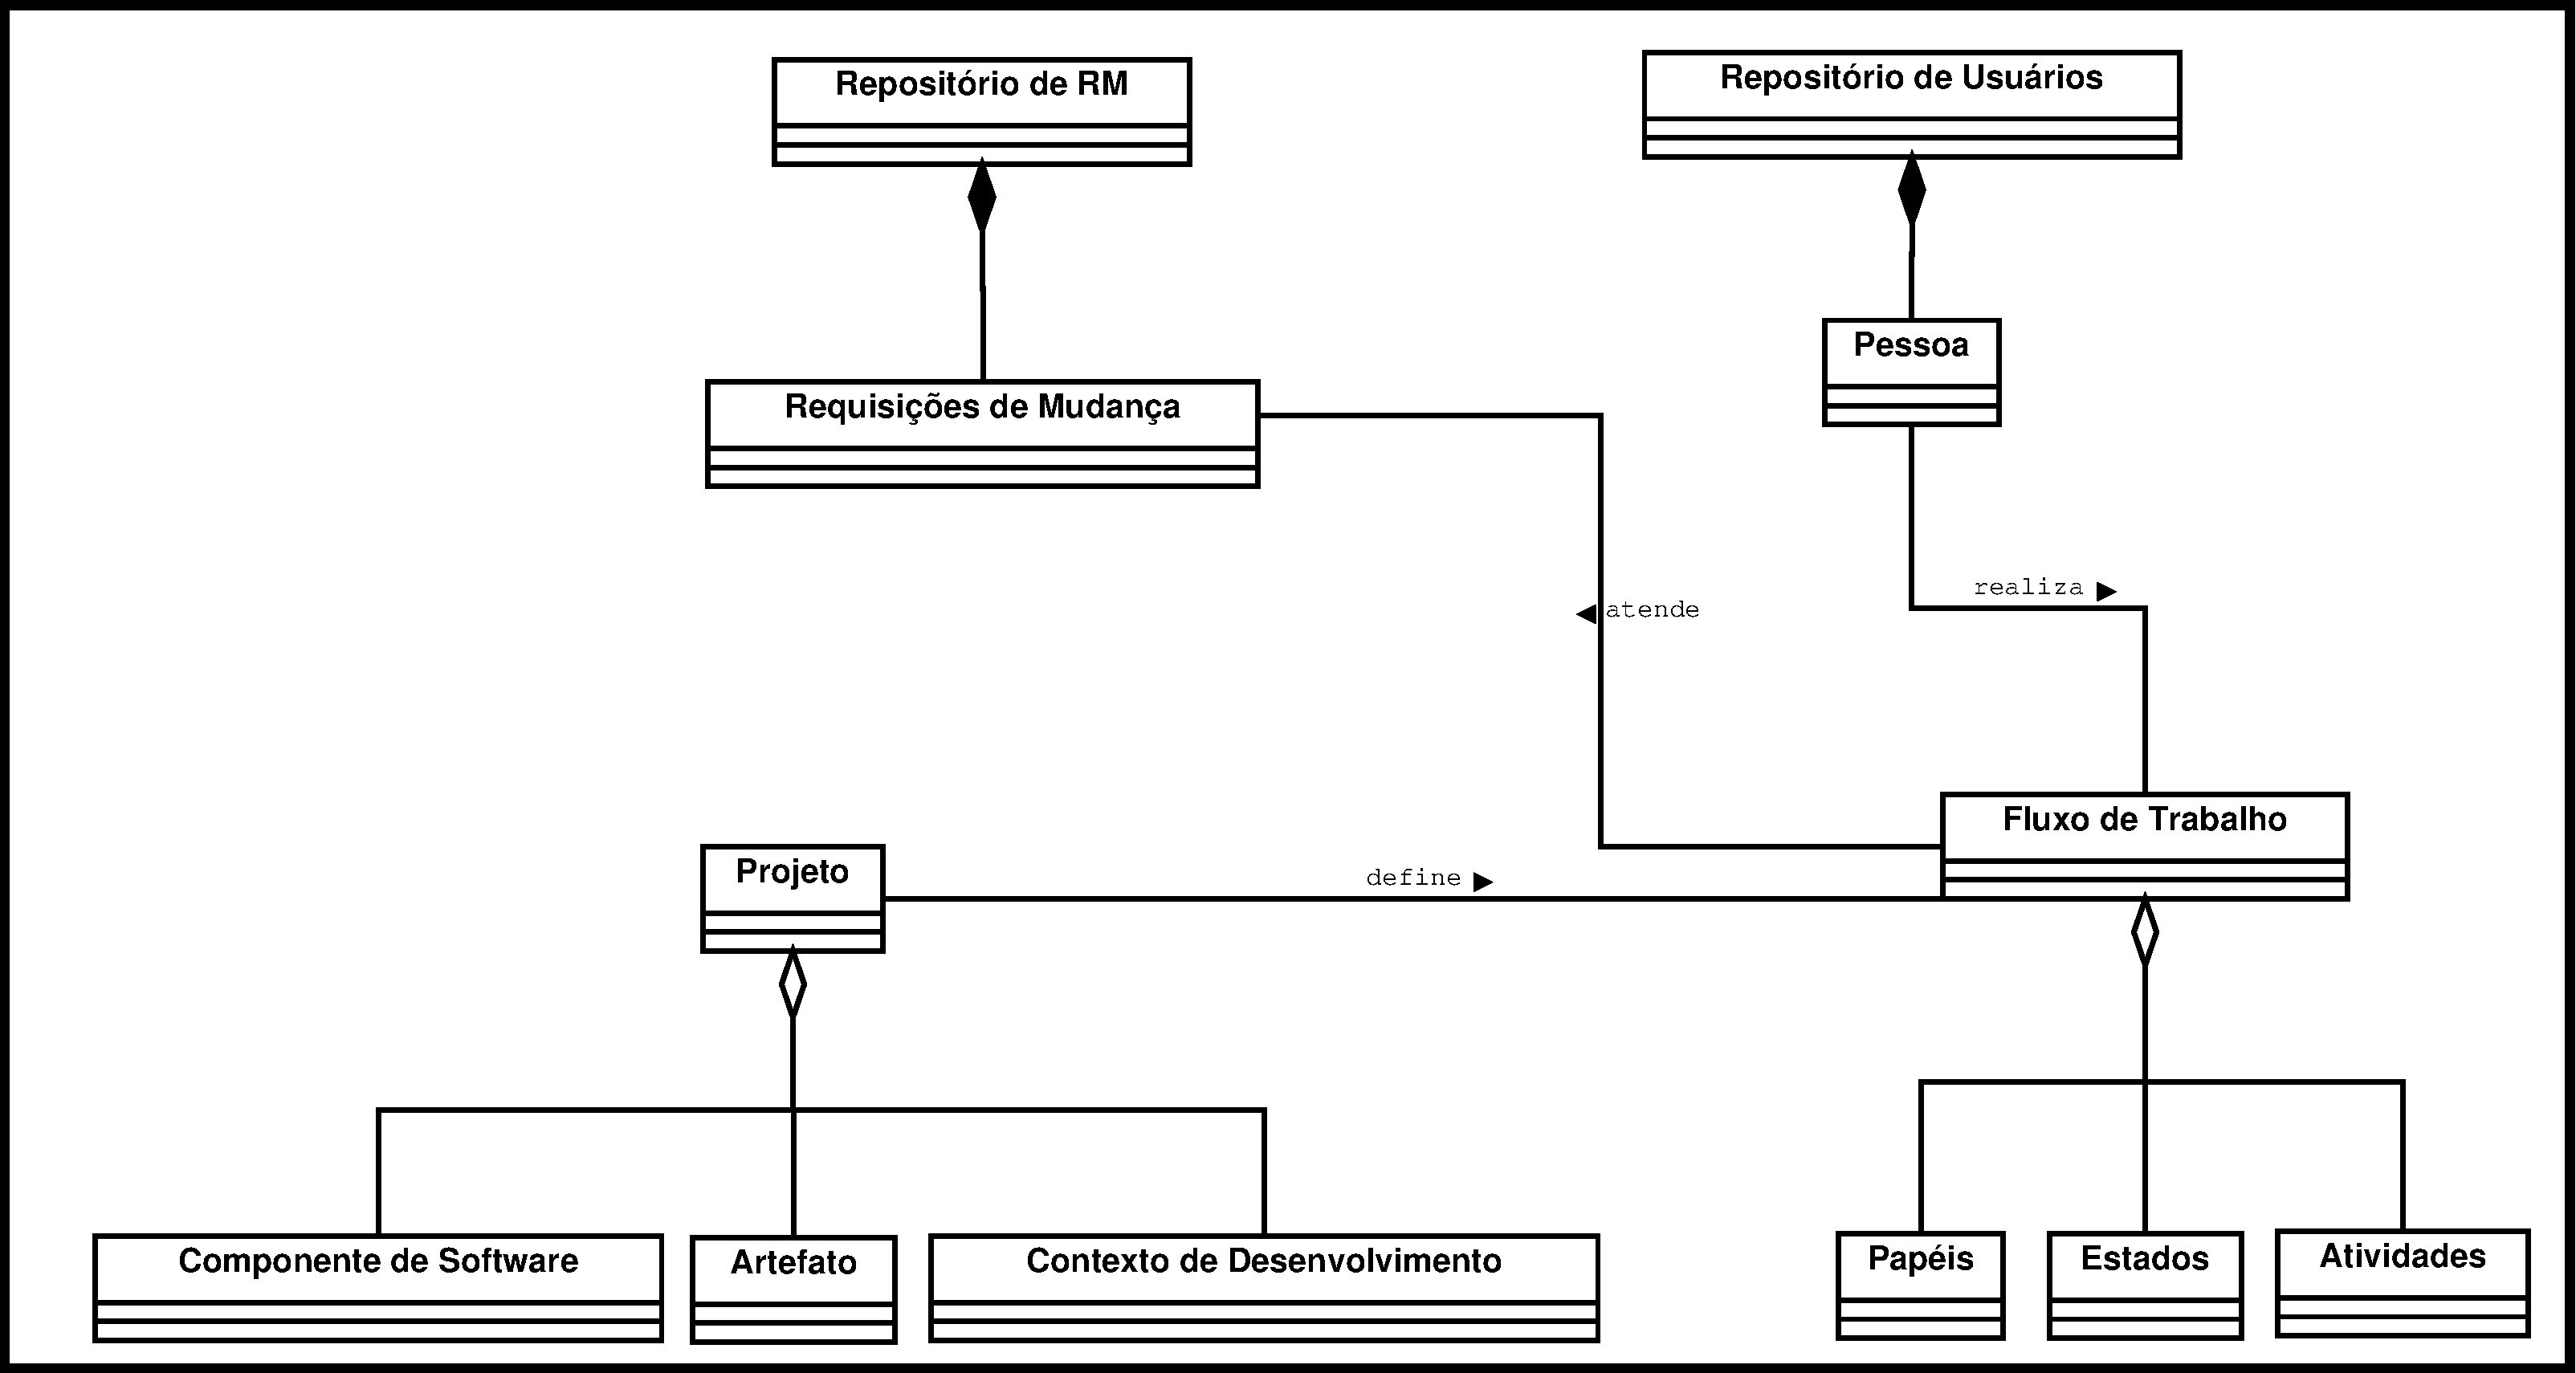
\includegraphics[width=1.15\linewidth]{./chapter-manutencao-software-visao-geral/img/diagrama-classe-conceitual-fgrm.pdf}
	\caption{Modelo conceitual do contexto de uma FGRM}
	\label{fig:diagrama-classe-conceitual-fgrm}
\end{figure}

Conforme exposto, as FGRM desempenham um papel que vai além de gerenciar as
Requisições de Mudança. Neste sentido, é importante estudar este tipo de
software em busca de como melhorá-los de modo a atender as diversas necessidades
dos seus usuários. Contudo, é importante avaliar as novas funcionalidades
propostas na li\-te\-ra\-tu\-ra ou ainda mesmo a melhoria das já existentes. Uma
possível forma de melhoria é através do uso de extensões. Na próxima seção
abordamos esta propriedade de algumas FGRM's que permitem a inclusão e
modificação de funcionalidades e comportamentos da ferramenta segundo as
necessidades do usuário.
\todoend

\subsection{Extensões em FGRM}
\label{subsec:manutencao_visao_geral_extensoes_fgrm}

Em determinados domínios de aplicação é interessante desenvolver produtos de
software com uma arquitetura que permita o sistema se adaptar às mudanças em
seus requisitos. Existe naturalmente a possibilidade de incluir as novas
funcionalidades dentro das já existentes no software, todavia, verificamos que
sistemas que permitem extensões apresentam os seguintes benefícios:

\begin{itemize}
	\item Extensibilidade: o software pode ser dinamicamente estendido mediante
		a inclusão de novos módulos de código que correspondem à novas
		características;
	\item Desenvolvimento em Paralelo: Quando os componentes não possui certas
		dependências eles podem ser desenvolvidos em paralelo por times
		diferentes;
	\item Simplicidade: uma  extensão; tipicamente tem uma única funcionalidade,
		desta forma permite um melhor foco para os desenvolvedores.
\end{itemize}

No escopo deste trabalho, uma extensão é um componente de software que adiciona
uma característica ou comportamento específico para um programa de
computador\footnote{\url{https://en.wikipedia.org/wiki/Plug-in_(computing)}}.
Cabe-nos ressaltar que o nossa definição de extensão incluí aquelas que não
estão acopladas ao código de determinada FGRM\@. Por exemplo, a funcionalidade
de atribuição de uma Requisição de Mudança a um ou mais desenvolvedor é inerente
às FGRM, segundo o nosso entendimento uma proposta de melhoria desta
funcionalidade mediante uma atribuição automatizada, por exemplo, será analisada
como extensão mesmo que ela não esteja efetivamente funcionando em alguma
FGRM\@. Vamos a\-na\-li\-sar as extensões de funcionalidade de forma
independente se ela é oferecida baseada nos mecanismos de extensão discutidos
nesta seção.

Verificamos na literatura alguns estudos em que as soluções propostas já se
tornaram extensões de determinadas FGRM. Como pode ser observado no Mapeamento
Sistemático realizado no Capítulo~\ref{ch:mapeamento-sistematico}, a
implementação da proposta do estudo em extensão de ferramenta não é o padrão
observado.

A extensão \textit{Buglocalizer}~\cite{Thung:2014:BIT:2635868.2661678} é uma
extensão para o Bugzilla que possibilita a localização dos arquivos do código
fonte que estão relacionados ao defeito relatado. A ferramenta extrai texto dos
campos de sumário e descrição de um determinado erro reportado no Bugzilla. De
maneira similar \textit{NextBug}~\cite{101186} também é uma extensão para o
Bugzilla que recomenda novos bugs para um desenvolvedor baseado no defeito que
ele esteja tratando atualmente. Em ambos os casos a extensão foi implementada
utilizando técnicas de Recuperação da Informação.

Os softwares que utilizam módulos de extensão têm aspectos de desenvolvimento e
de manutenção potencialmente distintos daqueles sem esta característica. Este
trabalho de mestrado faz uma contribuição na direção de uma melhor compreensão
deste contexto a partir da análise de aspectos específicos das FGRM's.

\section{Um Estudo sobre as Funcionalidades das FGRM's}
\label{sec:caracterizacao_ferramentas}

\subsection{Introdução}
\label{subsec:caracterizacao_intro}
Quando uma empresa ou um projeto de software de código aberto decide adotar uma
Ferramenta de Gerenciamento de Requisições de Mudança~-~FGRM um possível desafio
é encontrar aquela que melhor atenda suas necessidades. Um possível fundamento
de seleção é o conjunto de funcionalidades oferecidas pelo software. Outros
critérios podem envolver o custo e o suporte pós-venda da ferramenta. De maneira
relacionada, o pesquisador que estuda propostas de melhorias para as FGRM's pode
estar interessado em analisar o conjunto de funções que permita caracterizar
este tipo de software.

O número de FGRM's disponíveis quando esta dissertação foi escrita era bastante
elevado. Em uma inspeção inicial, verificamos a existência de mais de
\textit{50} ferramentas fornecidas comercialmente ou em código
aberto\footnote{\url{https://en.wikipedia.org/wiki/Comparison_of_issue-tracking_systems}}.
Apesar das diversas opções disponíveis, ao bem do nosso conhecimento,
desconhecemos estudos que avaliem sistematicamente as funcionalidades oferecidas
por este tipo de ferramenta. Entendemos que a partir de um conjunto
compartilhado de funções/comportamento seja possível caracterizar as FGRM's, ao
mesmo tempo que possibilita avaliar a contribuição de novas funcionalidades
propostas na li\-te\-ra\-tu\-ra, conforme discutido no
Capítulo~\ref{ch:mapeamento-sistematico}. Para alcançarmos este objetivo,
realizamos um estudo exploratório visando coletar as funcionalidades presentes
nas FGRM's. Um estudo exploratório está preocupado com a análise do objeto em
sua configuração natural e deixando que as descobertas surjam da própria
observação~\cite{wohlin2012experimentation}. Neste tipo de estudo nenhuma
hipótese é previamente definida.

O trabalho descrito neste capítulo consistiu na leitura da documentação
disponível na Internet de algumas FGRM's de modo a sistematizar as
funcionalidades o\-fe\-re\-ci\-das por cada ferramenta. As funções foram
coletadas e organizadas utilizando a técnica de Cartões de Classificação
(Sorting Cards)~\cite{5070993, rugg2005sorting}. Devido ao alto volume de
ferramentas disponíveis e ao esforço necessário para analisar a documentação de
todas elas, optamos por realizar este estudo com um conjunto de 6 ferramentas
que foram escolhidas com a ajuda de profissionais envolvidos em manutenção de
software. Através de um levantamento por meio de questionário(survey) onde os
profissionais definiram quais FGRM eram as mais representativas dentre uma lista
previamente definida. A representatividade neste contexto não está no número de
projetos que utiliza determinada ferramenta, mas pelas caraterísticas que o
software possui e que o torna diferenciável dentro do seu domínio.

\todobegin{Revisar este parágrafo para adequar a nova estrutura do capítulo}
Este capítulo está organizado da seguinte forma: na
Seção~\ref{sec:objetivo_do_capítulo} discutimos os objetos deste capítulo; na
Seção~\ref{sec:metodologia} apresentamos o método utilizado na condução do
estudo, em especial a técnica de Cartões de Ordenação e o levantamento realizado
com os profissionais para escolher as ferramenta do estudo.
\todoend

\subsection{Objetivo do Capítulo}
\label{subsec:caracterizacao_objetivo_do_capitulo}

O objetivo inicial deste capítulo é apresentar e discutir as principais
funcionalidades das FGRM's que dão suporte ao desenvolvimento e manutenção de
software. Tomando como ponto de partida um conjunto de sistemas definidos como
os mais relevantes escolhidos por meio de um levantamento(survey) com o uso de
questionário. Em um segundo momento, o foco foi caracterizar este tipo de
ferramenta tomando como base as funcionalidades oferecidas pelos softwares.
Conforme já exposto, a literatura em Manutenção de Software apresenta diferentes
nomenclaturas para este tipo de ferramenta (Sistema de Controle de Defeito~-~Bug
Tracking Systems, Sistema de Gerenciamento da Requisição~-~Request Management
System, Sistemas de Controle de Demandas (SCD)~-~Issue Tracking Systems), sem,
contudo, se preocupar em diferenciá-las.

Acreditamos que o resultado deste estudo permitirá compreender melhor este tipo
de software tomando como base o conjunto de funções que eles oferecem aos seus
usuários. Também será possível propor novas funcionalidades ou melhorias das
existentes tendo em vista a possibilidade de determinar o conjunto mínimo de
comportamentos deste tipo de ferramenta.

\subsection{Metodologia}
\label{subsec:metodologia}

A fim de determinarmos o conjunto de funcionalidades das FGRM's realizamos um
estudo exploratório dividido em três etapas que estão listadas a seguir. O
resultado obtido em etapa foi utilizado para subsidiar as atividades do etapa
subsequente. O início de uma nova fase do trabalho era precedido de uma
avaliação geral com o objetivo de verificar possíveis inconsistências e
avaliação das lições aprendidas.

\begin{enumerate}[(i)]
	\item Seleção das Ferramentas
	\item Inspeção da Documentação
	\item Agrupamento das Funcionalidades
\end{enumerate}

\subsubsection{Seleção das Ferramentas}
\label{subsubsec:selecao-ferramentas}

A primeira etapa consistiu da definição das ferramentas que seriam utilizadas no
estudo. A partir de uma pesquisa na Internet obtivemos um conjunto inicial de 50
ferramentas\footnote{\url{https://en.wikipedia.org/wiki/Comparison_of_issue-tracking_systems}}
que podem ser visualizadas no Anexo~\ref{ch:app-lista-fgrm}. Devido ao esforço
necessário e a dificuldade de realizar a análise em cada uma daquelas
ferramentas, optamos por escolher um subconjunto de sistemas que fossem mais
representativos, tomando como base a opinião de profissionais envolvidos em
manutenção e desenvolvimento de software. A representatividade neste caso
corresponde a opinião do profissional sobre notoriedade que a ferramenta possui
dentro do seu domínio de aplicação em comparação com as demais que lhe foram
apresentadas ou outras do qual o profissional tenha prévio conhecimento.

\subsubsection{Desenho da Pesquisa com Profissionais}
\label{ssub:metodologia_desenho_da_pesquisa_com_profissionais}

A opinião dos profissionais foi obtida mediante a realização de uma pesquisa de
opinião (survey~\cite{wohlin2012experimentation}) realizada com o uso de um
formulário eletrônico. O formulário foi estruturado em duas partes principais: a
formação de base do participante (background) e a avaliação das ferramentas. Na
primeira parte estávamos interessados em conhecer as características do
respondente. Esta informação é relevante tendo em vista que, como descreveremos
a seguir, o questionário foi replicado em três grupos distintos de
profissionais. Na segunda parte apresentamos as ferramentas e foi solicitado aos
participantes que avaliassem a relevância de cada uma delas através de questões
de múltipla escolha. As opções de respostas foram estruturadas em escala do tipo
Likert~\cite{robbins2011plotting}. Também foi disponibilizado aos participantes
um campo de texto livro no qual era possível informar FGRM's que ele entenda por
relevante, mas que não estava na lista que lhe foi apresentada. Para estas
ferramentas que foram citadas de forma espontânea foi atribuído um grau de
importância igual ``Muito relevante'' conforme Tabela~\ref{tab:graus_relevancia}
no cálculo da métrica de relevância conforme
equação~\ref{eq:escolha_ferramenta}.

Antes da efetiva aplicação do questionário em alguma amostra da população do
estudo, o documento foi validado em um processo de três etapas. Na primeira
parte foi solicitado a dois pesquisadores experientes da área de Engenharia de
Software que avaliassem o formulário. A partir das sugestões obtidas dos
pesquisadores foram realizadas adequações no documento. Após as alterações uma
nova versão do formulário foi enviada para dois profissionais envolvidos
diretamente em manutenção de software. O critério utilizado para seleção dos
profissionais foi o tempo de experiência com desenvolvimento e manutenção de
software, que era em média de 10 anos. O formulário foi modificado com as
sugestões dos profissionais e isso finaliza a segunda etapa de validação. A
última etapa consistiu na realização de um piloto com dez profissionais que
trabalham em um setor de uma empresa pública de informática. Os profissionais
tiveram que preencher o questionário, contudo, foram adicionadas questões
adicionais onde era possível inserir sugestões de melhoria. O resultado deste
processo de validação é o questionário presente no
Anexo~\ref{ch:app-form-selecao-ferramentas}. Como o público-alvo do questionário
poderia incluir desenvolvedores de diferentes nacionalidades foi construído uma
versão em língua inglesa do formulário.

A população de interesse deste levantamento é o conjunto de profissionais
envolvidos em manutenção de software. Naturalmente é difícil definir o tamanho e
características desta população de modo a mensurar uma amostra significativa.
Neste sentido, visando minimizar enviesamento deste estudo, o questionário
foi replicado em três grupos:

\begin{description}
	\item[Grupo 01:] Profissionais de empresa pública e privada de
			desenvolvimento e manutenção de software.
	\item[Grupo 02:] Profissionais que contribuem em projetos de
		código aberto
	\item[Grupo 03:] Profissionais que participam de grupos de
		interesse sobre desenvolvimento e manutenção de software em uma rede
		social profissional (LinkedIn) ou aqueles que participam de discussão
		sobre este assunto em uma rede social (Stack Overflow).
\end{description}

Os participantes que compõem cada grupo foram escolhidos conforme critérios que
são detalhados no Capítulo~\ref{ch:pesquisa-profissionais}. A reutilização desta
base de desenvolvedores se deu por conta de ambos os estudos compartilharem a
mesma população de interesse, podendo neste caso compartilhar a mesma amostra.

\subsubsection{Critérios de Seleção}
\label{ssub:metodologia_criterios_selecao}

Com base nos dados obtidos da pesquisa com os profissionais, as FGRM's foram
classificadas como \textit{''ferramentas''} e \textit{''serviços da internet''}
utilizando a documentação do software. O primeiro grupo representa os softwares
que são capazes de serem implantados na infraestrutura do seu cliente e permite
algum grau de personalização de pelo menos um dos componentes, como por exemplo,
o banco de dados utilizado. No segundo grupo estão os software que ofertam a
gerência das RM's mediante uma arquitetura do tipo Software como Serviço
(Software as Service)~\cite{fox2013engineering}, onde certos tipos de alterações
no comportamento do software são mais restritas. Acreditamos que ao escolher
ferramentas dos dois tipos iremos cobrir uma grande parte do domínio de
aplicação das FGRM's. Optamos por escolher~\textit{06 ferramentas} para o
estudo, sendo três de cada um dos grupos.

Para seleção das ferramentas utilizados a formula apresentada na
Equação~\ref{eq:escolha_ferramenta}.  Atribuímos a métrica $r_i$ que representa
a relevância de determinada ferramenta $f_i$. A métrica é calculada somando a
frequência de cada um dos graus de relevância apresentado na
Tabela~\ref{tab:graus_relevancia} multiplicado pela pelo grau de relevância
descrito na mesma tabela.

\begin{equation}
\label{eq:escolha_ferramenta}
r_i = \sum_{i=1}^{n} f_i \times w_j
\end{equation}

A documentação de algumas ferramentas, em especial aquelas que adotam uma
arquitetura cliente/servidor e necessitam de um certo grau de administração,
dividem as funcionalidades do software entre aquelas com foco no usuário final e
ad\-mi\-nis\-tra\-do\-res. Nestes casos, optamos por coletar as funcionalidades
cujo o foco seja o usuário da FGRM, tendo em vista que administradores deste
tipo de software não estarem entre no público-alvo desta dissertação.

\begin{table}[htb]
\centering
	\resizebox{0.6\linewidth}{!}{%
\begin{tabular}{|clc|}
\hline
\textbf{$j$} & \textbf{Grau de Relevância} & \textbf{Peso($w_j$)} \\ \hline
1 & Não conheço a ferramenta & 1 \\
2 & Nada relevante & 2 \\
3 & Pouco relevante & 3 \\
4 & Pouco relevante & 4 \\
5 & Muito relevante & 5 \\ \hline
\end{tabular}%
}
\caption{Graus de Relevância}
\label{tab:graus_relevancia}
\end{table}

\subsubsection{Inspeção da Documentação}
\label{subsec:inspecao_doumentacao}

Nesta etapa do trabalho realizamos a leitura do material disponível na Internet
para cada uma das ferramentas que foram selecionadas conforme critérios
descritos na Subseção~\ref{ssub:metodologia_criterios_selecao}. Entre estes
materiais utilizamos manuais do usuário e do desenvolvedor e notas de
lançamento. Para cada uma das FGRM's optamos por estudar a última versão estável
do software a fim de analisarmos o que há de mais novo disponível aos usuários.
A Tabela~\ref{tab:fgrm-docs} apresenta as ferramentas analisadas e o elo de
ligação para cada documentação utilizada neste estudo. Para aquelas ferramentas
que apresentam documentação em mais de um i\-di\-o\-ma optamos por utilizar
aquela escrita em inglês por entendermos ser a que esteja mais atualizada.

\begin{table}[htpb]
\centering
\resizebox{\textwidth}{!}{%
\begin{tabular}{|l|l|}
\hline
\multicolumn{1}{|c|}{\textbf{Nome da Ferramenta}} & \multicolumn{1}{c|}{\textbf{Elo de Ligação}} \\ \hline
Bugzilla & \url{https://www.bugzilla.org/features/} \\
Github Issue Tracking System & \url{https://github.com/blog/411-github-issue-tracker} \\
Github Issue Tracking System & \url{https://github.com/features} \\
Github Issue Tracking System & \url{https://guides.github.com/features/issues/} \\
Gitlab Issue Tracking System & \url{http://docs.gitlab.com/ce/user/project/labels.html} \\
Gitlab Issue Tracking System & \url{https://about.gitlab.com/2016/08/22/announcing-the-gitlab-issue-board/} \\
Gitlab Issue Tracking System & \url{https://about.gitlab.com/solutions/issueboard/} \\
Gitlab Issue Tracking System & \url{https://docs.gitlab.com/ee/user/project/description\_templates.html} \\
Gitlab Issue Tracking System & \url{https://docs.gitlab.com/ee/user/project/issues/automatic\_issue\_closing.html} \\
Gitlab Issue Tracking System & \url{https://docs.gitlab.com/ee/workflow/issue\_weight.html} \\
Gitlab Issue Tracking System & \url{https://docs.gitlab.com/ee/workflow/milestones.html} \\
Gitlab Issue Tracking System & \url{https://docs.gitlab.com/ee/workflow/time\_tracking.html} \\
JIRA & \url{https://br.atlassian.com/software/jira/features} \\
MantisBT & \url{https://www.mantisbt.org/wiki/doku.php/mantisbt:features} \\
Redmine & \url{http://www.redmine.org/projects/redmine/wiki/Features} \\ \hline
\end{tabular}%
}
\caption{Documentações utilizadas no processo de coleta de dados.}
\label{tab:fgrm-docs}
\end{table}

Os dados obtidos da leitura do material disponíveis para cada ferramenta foram
sistematizados por meio de técnica denominada \textit{Cartões de
	Classificação~-~Sorting Cards}. Cartões de Classificação é um técnica de
elicitação de conhecimento, de baixo custo e com foco no usuário, largamente
utilizada em arquitetura informacional para criar modelos mentais e derivar
taxonomias da entrada utilizada~\cite{just2008towards}. Ela envolve a
categorização de um conjunto de cartões em grupos distintos de acordo com algum
critério previamente definido~\cite{mcgee2009software}. O estudo de Maiden e
outros~\cite{maiden1996acre} sugere que a técnica de Cartões de Classificação é
uma das mais úteis para aquisição de conhecimento de dados, em contraste ao
conhecimento de comportamento ou de processo.

Existem três principais fases dentro do processo de classificação dos cartões:
($i$) preparação, no qual participantes ou o conteúdo dos cartões são selecionados;
($ii$) execução, onde o cartões são organizados em grupo significativos com um
título que o descreve; e por fim, ($iii$) análise, no qual os cartões são
sistematizados para formar hierarquias mais abstratas que são usadas para
deduzir resultados. No processo tradicional de Cartões Ordenados cada declaração
realizada por um participante resulta na criação de exatamente um único
cartão~\cite{just2008towards}. Contudo, no nosso caso, foi realizada a divisão
da documentação da ferramenta por cada funcionalidade encontrada. Neste sentido,
cada funcionalidade obtida mediante a inspeção da documentação foi mapeada em
único cartão.

Os cartões foram organizados de modo que continham o nome e a versão da
ferramenta analisada; a URL da documentação utilizada; o nome da funcionalidade
coletada, que consiste de uma descrição breve conforme existente na
documentação; descrição detalhada da funcionalidade, cujo objetivo é facilitar o
processo de agrupamento que será descrito na próxima seção. O
Anexo~\ref{ch:app-form-cartoes-ordenados} apresenta um formulário que representa
os cartões utilizados neste estudo. Nas Figura~\ref{fig:documentacao_bugzilla}
e~\ref{fig:exemplo_cartao_ordenado} é possível visualizar, respectivamente, a
documentação de uma funcionalidade da FGRM Bugzilla e o cartão que foi gerado
para a mesma.

\todobegin{Incluída figuras para incluir a coleta dos dados da documentação das
ferramentas}
\begin{figure}[htpb]
	\centering
	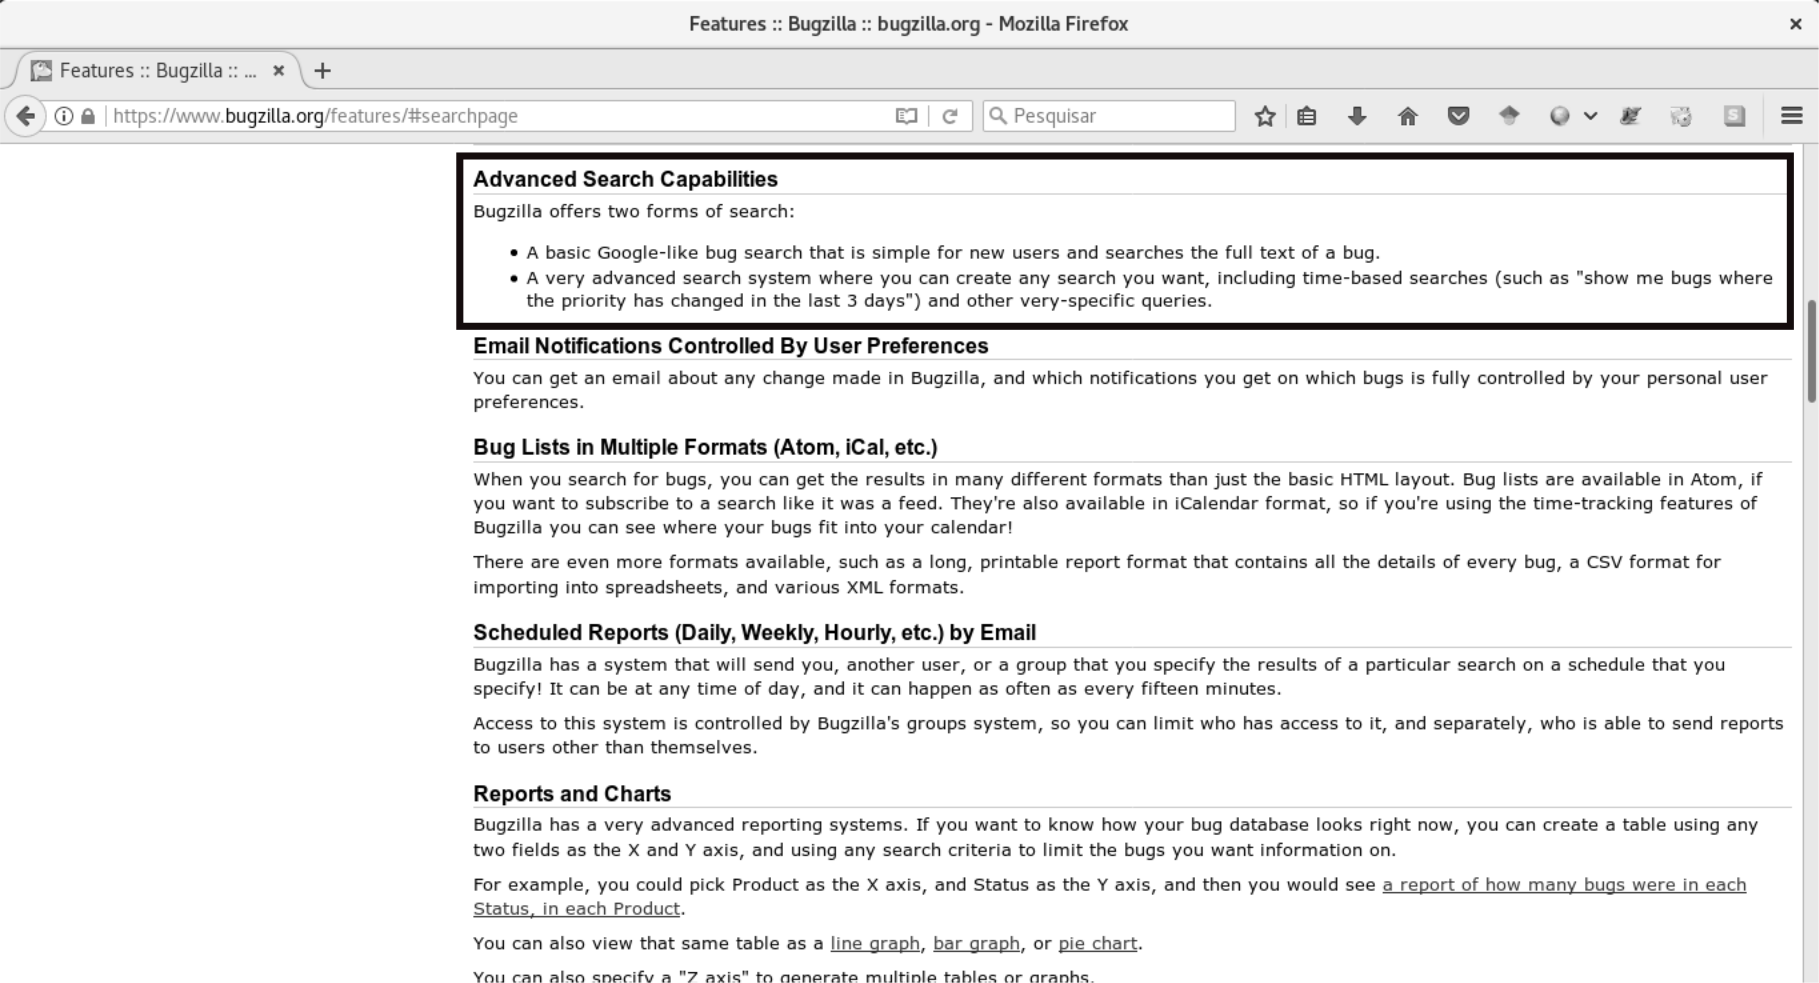
\includegraphics[width=0.8\linewidth]{./chapter-estudo-funcionalidades-fgrm/img/documentacao_bugzilla.png}
	\caption{Exemplo de documentação de uma funcionalidade da FGRM Bugzilla}
	\label{fig:documentacao_bugzilla}
\end{figure}

\begin{figure}[htpb]
	\centering
	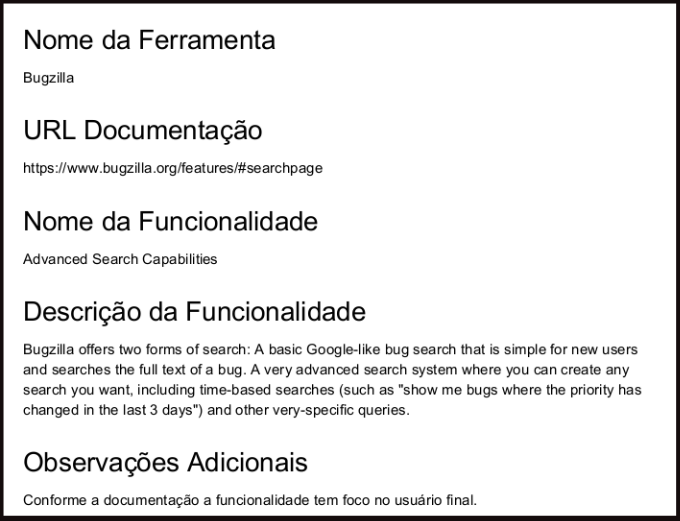
\includegraphics[width=0.8\linewidth]{./chapter-estudo-funcionalidades-fgrm/img/exemplo_cartao_ordenado.png}
	\caption{Exemplo de um cartão ordenado para uma funcionalidade da FGRM
		Bugzilla}
	\label{fig:exemplo_cartao_ordenado}
\end{figure}
\todoend

\subsubsection{Agrupamento das Funcionalidades}
\label{subsec:agrupamento_fucionalidades}

Esta etapa tem por objetivo agrupar as funcionalidades que aparecem com
nomenclatura distintas em diferentes ferramentas, mas que apresentam o mesmo
significado. Cabe ressaltar que o agrupamento de algumas funcionalidades pode
depender de uma análise subjetiva do responsável pela atividade. Neste sentido,
a fim de evitar algum tipo de viés o agrupamento foi realizado em duas etapas:

\begin{description}
	\item[Análise Individual] Neste etapa o autor e um outro especialista
		realizam de forma separada os agrupamentos que acharem necessários.
	\item[Anaĺise Compartilhada] Em um segundo momento tanto o autor quanto o
		es\-pe\-ci\-a\-lis\-ta discutem as possíveis divergências até que um
		consenso seja obtido.
\end{description}

Após o processo de agrupamento foi possível realizar a categorização das
funcionalidades das ferramentas. Os resultados do processo de agrupamento são
apresentados e discutidos nas próximas seções.

\subsection{Resultados}
\label{sec:resultados}

Nesta seção iniciaremos apresentando o resultado do processo de escolha das
ferramentas que foi realizado mediante um levantamento com questionário.
Começamos por apresentar o perfil dos participantes e em seguida exibimos as
categorias resultantes do processo de ordenamento dos cartões.

\subsubsection{Perfil dos Participantes}
\label{ssub:Perfil dos Participantes}
Ao final do levantamento realizado com profissionais obtivemos um total de
\textit{52} respostas. Os profissionais que participaram são em sua maioria
desenvolvedores conforme pode ser verificado na
Figura~\ref{fig:grafico_escolha_ferramentas_funcao_participantes}.

\begin{figure}[htpb]
	\centering
	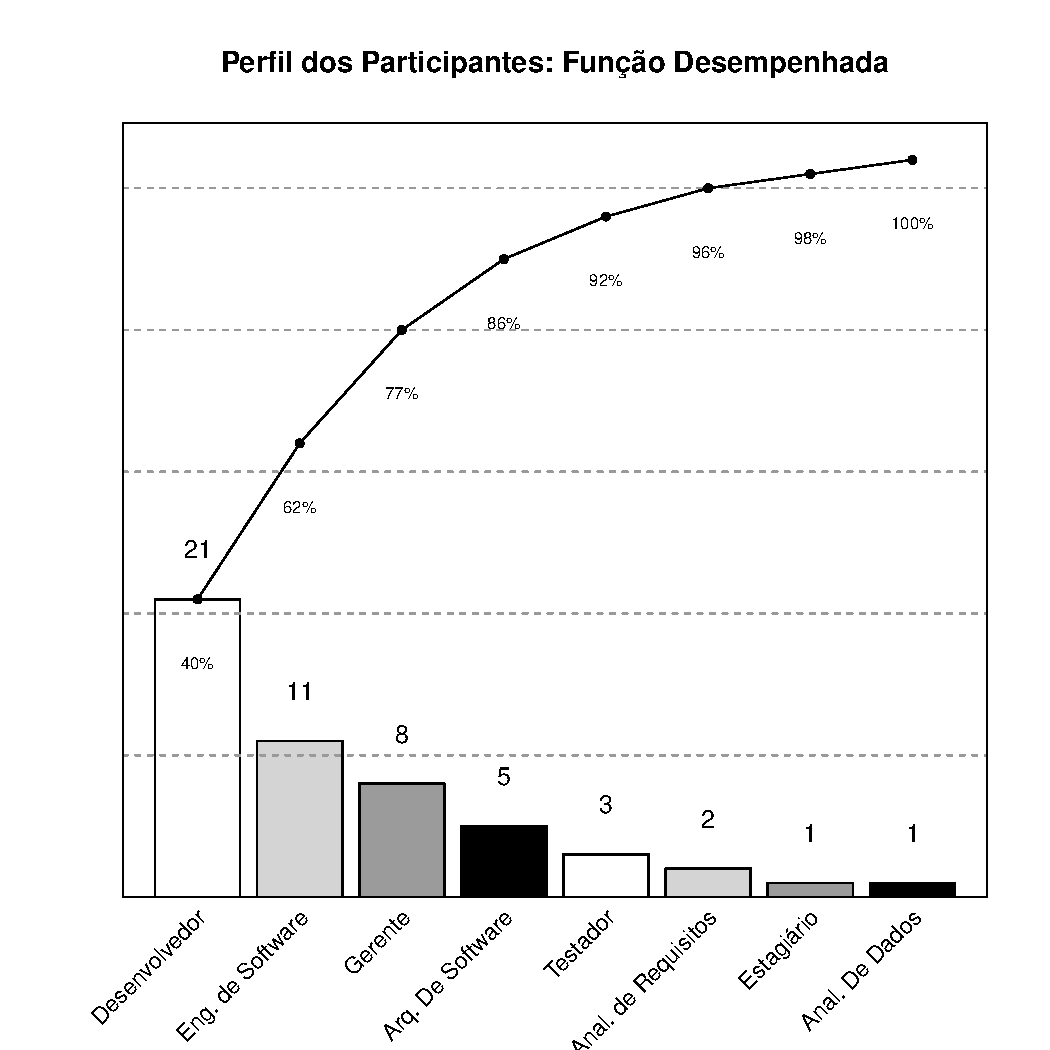
\includegraphics[width=0.8\linewidth]{./chapter-estudo-funcionalidades-fgrm/img/grafico_escolha_ferramentas_funcao_participantes.pdf}
	\caption{Funções desempenhadas pelos participantes}
	\label{fig:grafico_escolha_ferramentas_funcao_participantes}
\end{figure}

O grupo de respondentes também incluem Engenheiros de Software, Gerentes de
Equipe e Arquitetos de Software que, junto com os Desenvolvedores, representam
mais de 80\% do total. Com relação a experiência verificamos que a maior parte
possui entre 3 e 10 anos, conforme pode ser verificado pela
Figura~\ref{fig:grafico_escolha_ferramentas_tempo_experiencia}.

\begin{figure}[htpb]
	\centering
	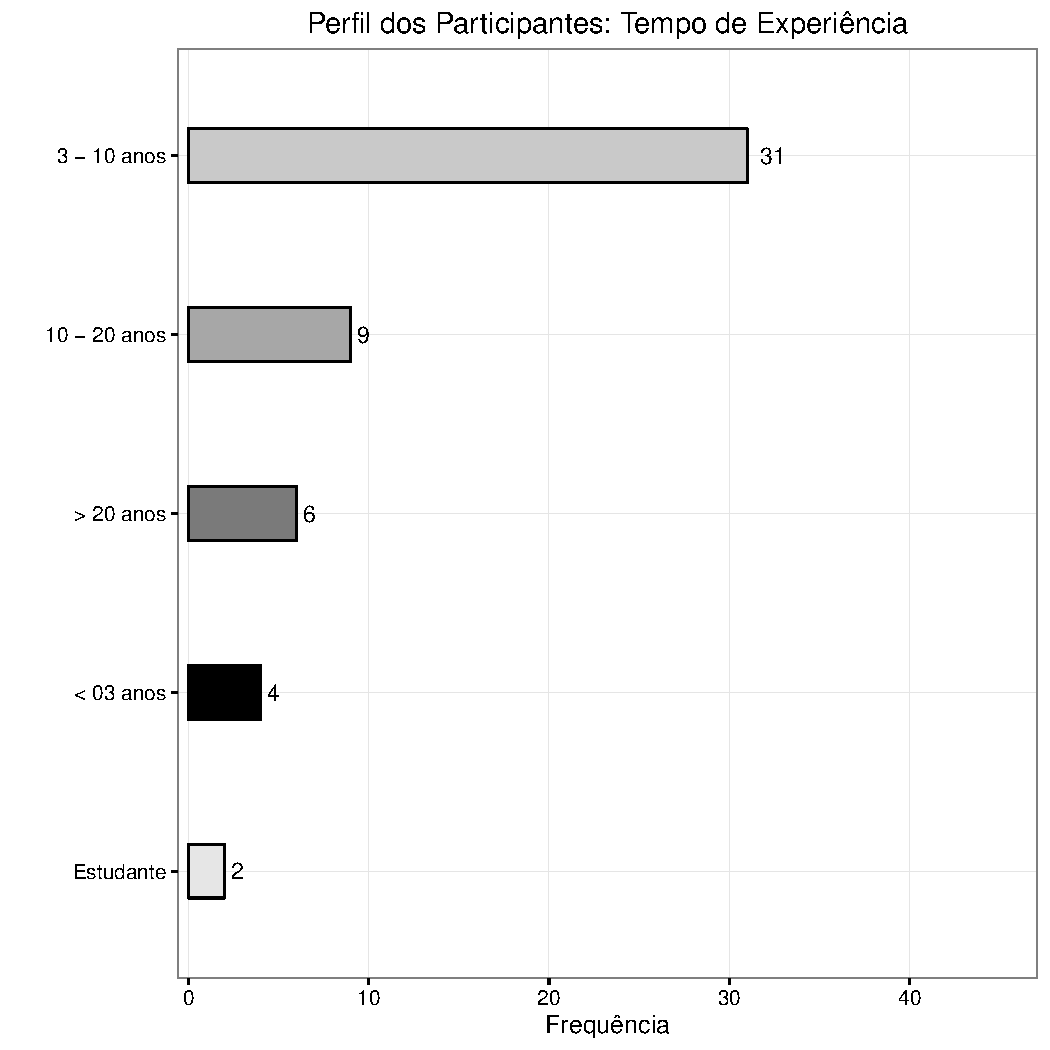
\includegraphics[width=0.8\linewidth]{./chapter-estudo-funcionalidades-fgrm/img/grafico_escolha_ferramentas_tempo_experiencia.pdf}
	\caption{Tempo de Experiência}
	\label{fig:grafico_escolha_ferramentas_tempo_experiencia}
\end{figure}

Com relação ao tamanho da equipe em que os participantes fazem parte,
verificamos uma prevalência de equipes de médio ( mais do que 10 membro) e
pequenas (2 a 5 membros) porte. A
Figura~\ref{fig:grafico_escolha_ferramentas_tamanho_equipe} exibe o tamanho da
equipe dos participantes. Por sua vez, estas equipes estão predominantemente em
empresas privadas de software. Com relação ao local de trabalho verificamos
ainda que o segundo posto em número par\-ti\-ci\-pan\-tes ficou para empresas
que pertencem ao setor governamental. Esta distribuição pode ser visualizada na
Figura~\ref{fig:grafico_escolha_ferramentas_local_trabalho}.

\begin{figure}[htpb]
	\centering
	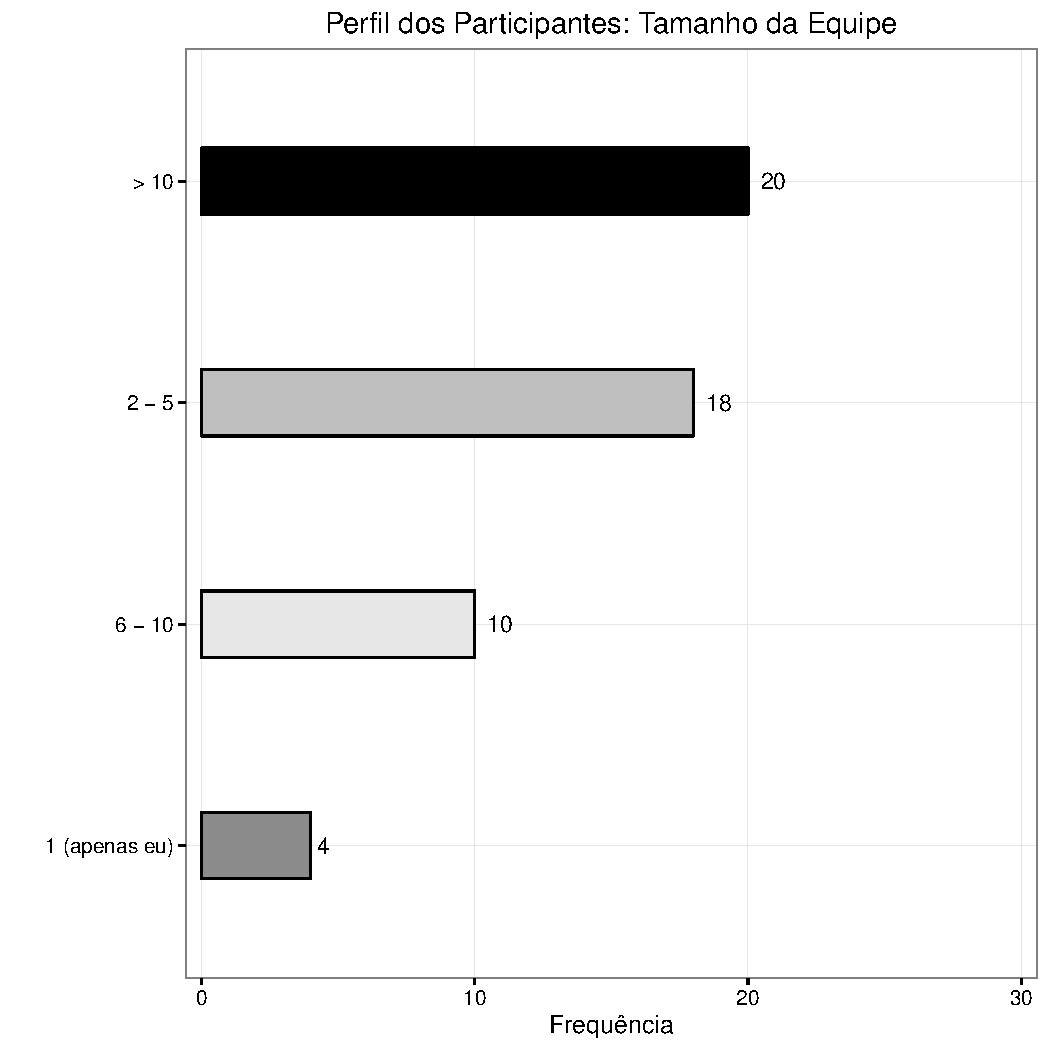
\includegraphics[width=0.8\linewidth]{./chapter-estudo-funcionalidades-fgrm/img/grafico_escolha_ferramentas_tamanho_equipe.pdf}
	\caption{Tamanho da Equipe}
	\label{fig:grafico_escolha_ferramentas_tamanho_equipe}
\end{figure}

Em geral, podemo caracterizar o participante típico como um desenvolvedor entre
três e dez anos de experiência trabalhando em uma empresa privada de
desenvolvimento de software que com uma equipe de aproximadamente dez membros.
Segundo o nosso entendimento, como este perfil um profissional tem o
conhecimento necessário para nos ajudar no processo de escolha das ferramentas.

\begin{figure}[htpb]
	\centering
	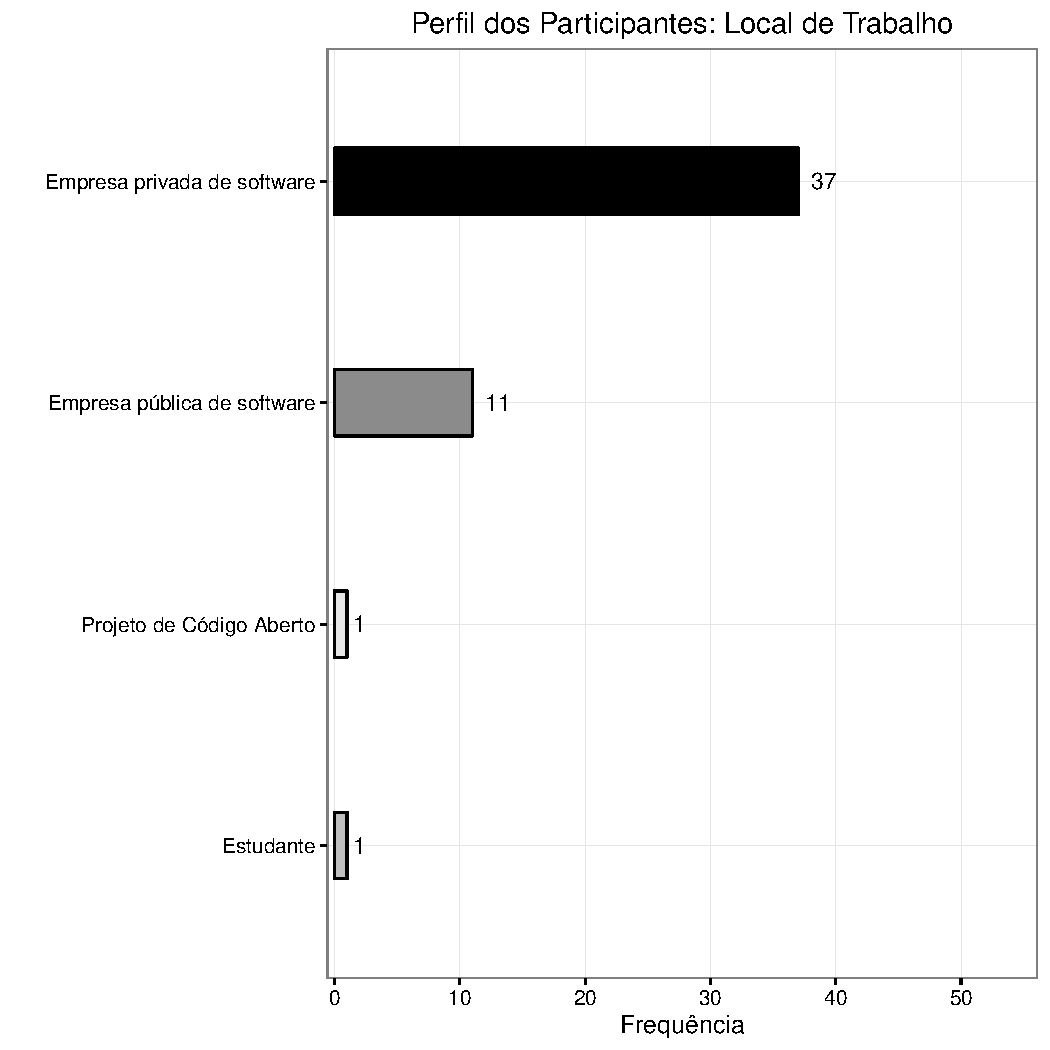
\includegraphics[width=0.8\linewidth]{./chapter-estudo-funcionalidades-fgrm/img/grafico_escolha_ferramentas_local_trabalho.pdf}
	\caption{Local de trabalho}
	\label{fig:grafico_escolha_ferramentas_local_trabalho}
\end{figure}

\subsubsection{Ferramentas Escolhidas}
\label{subsec:resultados_ferramentas_escolhidas}

Utilizando a Equação~\ref{eq:escolha_ferramenta} obtivemos as ferramentas
apresentas na Tabela~\ref{tab:ferramenta_utilizadas_estudo}. Conforme pode ser
observado foi escolhido três softwares de cada tipo (ferramenta e serviço da
Internet). É importante perceber que as FGRM's \textit{Github e Gitlab} não
estavam na lista inicial, contudo, apareceram neste resultado final. Isso
decorre  de atribuímos o maior peso ($w_i = 5$) para aquelas ferramentas que
foram citadas pelos participantes de maneira espontânea.  Neste caso, devido a
frequência que estas ferramentas elas acabaram escolhidas.

\begin{table}[htb]
\centering
\caption{Ferramentas utilizados no estudo}
\label{tab:ferramenta_utilizadas_estudo}
\resizebox{\textwidth}{!}{%
\begin{tabular}{|lccl|}
\hline
\multicolumn{1}{|c}{\textbf{Ferramenta}} & \textbf{Classificação} & \textbf{Versão} & \multicolumn{1}{c|}{\textbf{URL}}      \\ \hline
Bugzilla                                 & Ferramenta             & 5.0.3           & https://www.bugzilla.org               \\
Mantis Bug Tracker                       & Ferramenta             & 1.3.2           & https://www.mantisbt.org               \\
Redmine                                  & Ferramenta             & 3.3.1           & http://www.redmine.org/                \\
JIRA Software                            & Serviço                & 7.2.4           & https://br.atlassian.com/software/jira \\
Github Issue System             & Serviço                & \@-\@           & https://github.com/                    \\
Gitlab Issue Tracking System             & Serviço                & \@-\@           & https://gitlab.com/                    \\ \hline
\end{tabular}%
}
\end{table}


\subsubsection{Espectro de Funcionalidades das FGRM's}
\label{subsec:categorizacao_ferramentas}

\todobegin{Incluída uma classificação das funcionalidades nas dimensões Gestão da
RM, Ferramenta e Processo}

Após a inspeção da documentação e validação dos dados obtivemos um total de 123
cartões. Nós sistematizamos os cartões manualmente tendo em vista que não
existem ferramentas ou métodos capazes de automatizar o processo de construção
de hi\-e\-rar\-qui-\-as. Como o nosso objetivo é derivar tópicos a partir de um
conjunto inicial de cartões, optamos por realizar um \textit{ordenamento
	aberto}. Neste tipo de abordagem, os grupos são estabelecidos durante o
processo de classificação dos cartões em oposição a outra forma de utilização da
técnica onde a sistematização dos cartões ocorre com base em grupos
pré-determinados. Ao final do processo compilamos os tópicos de modo a construir
um espectro de funcionalidades para as FGRM que pode observado na
Figura~\ref{fig:diagrama-espectro-funcionalidades-fgrm}, no qual temos três
dimensões de funcionalidades que são compostas por diferentes categorias de
funcionalidades.

\begin{figure}[htpb]
	\centering
	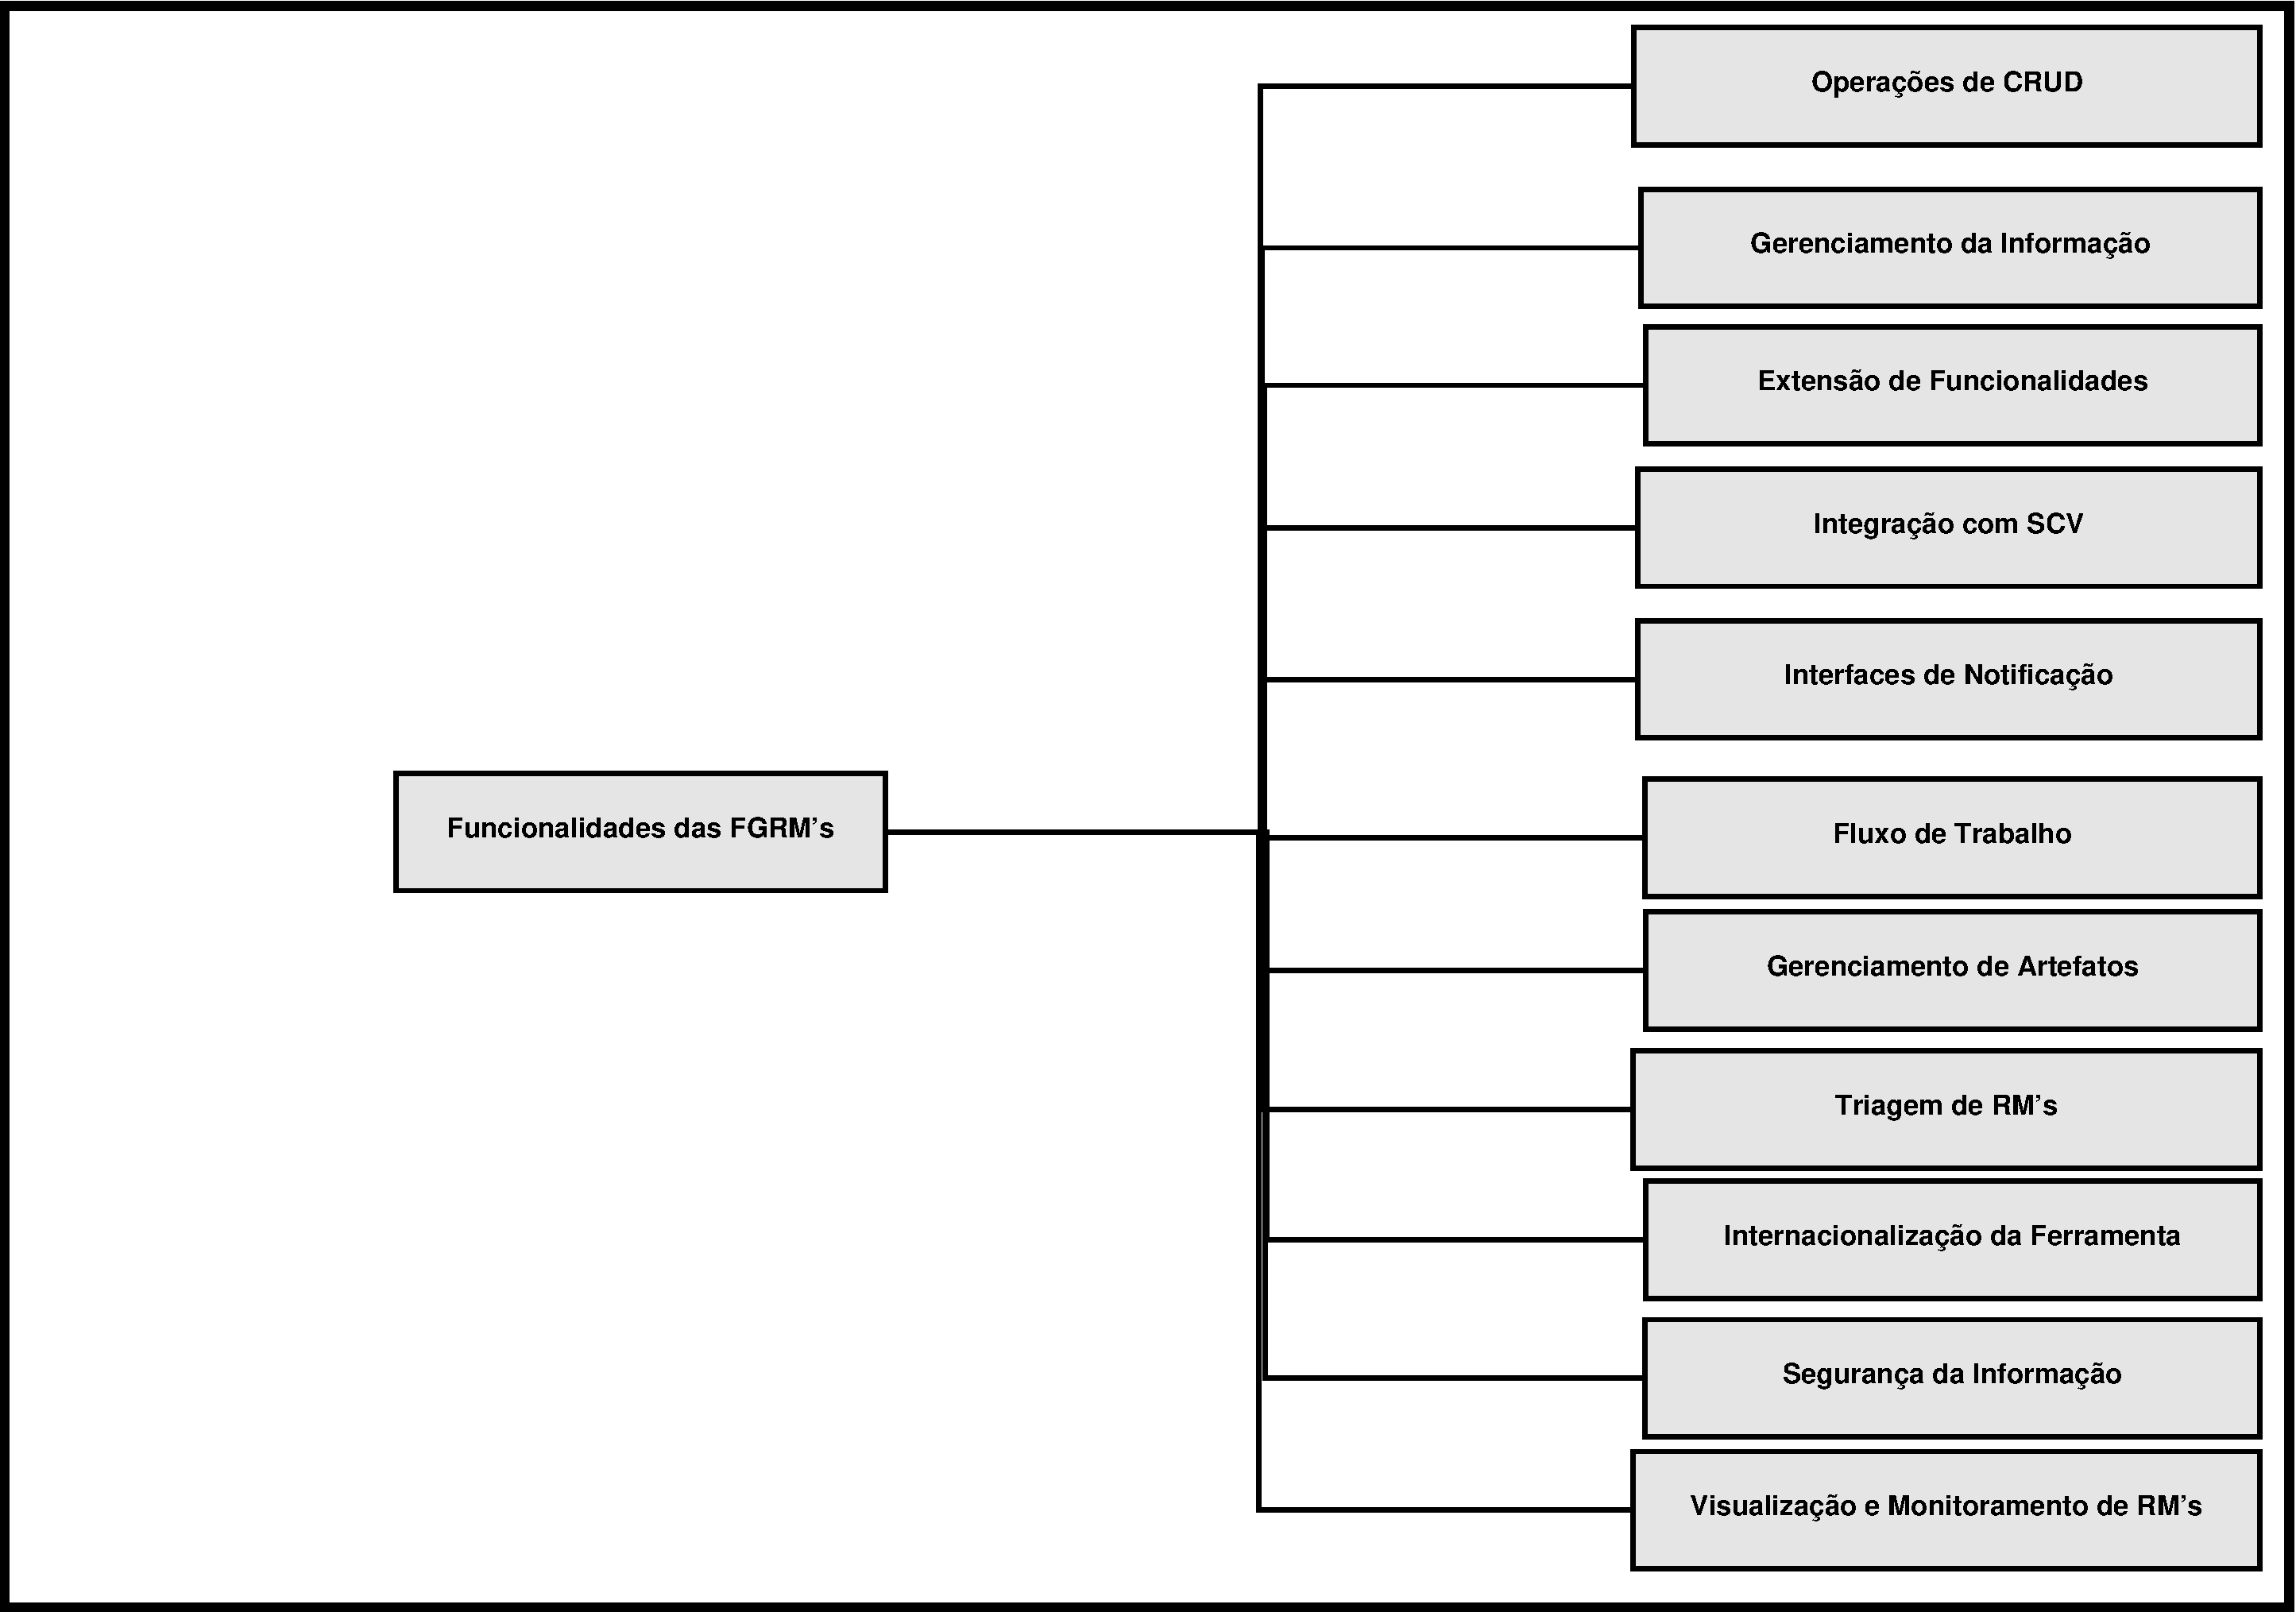
\includegraphics[width=1.15\linewidth]{./chapter-estudo-funcionalidades-fgrm/img/diagrama-espectro-funcionalidades-fgrm.pdf}
	\caption{Dimensões técnicas de uma FGRM}
	\label{fig:diagrama-espectro-funcionalidades-fgrm}
\end{figure}

A figura foi construída com base nas categorias de funcionalidades exibidas na
Tabela~\ref{tab:freq_categorias_cartoes} onde é possível verificar ainda a
frequência que cada uma das categorias apareceu no conjunto de cartões
coletado.

\begin{table}[htpb]
\centering
\resizebox{.7\textwidth}{!}{%
\begin{tabular}{|l|c|}
\hline
\multicolumn{1}{|c|}{\textbf{Categoria de Funcionalidades}} & \textbf{Frequência} \\ \hline
Operações de CRUD & 24 \\
Visualização e Monitoramento de RM's & 22 \\
Segurança da Informação & 17 \\
Fluxo de Trabalho & 15 \\
Interfaces de Notificação & 13 \\
Extensão de Funcionalidades & 8 \\
Triagem de RM's & 6 \\
Gerenciamento de Artefatos & 6 \\
Integração com Sistemas de Controle de Versão & 4 \\
Gerenciamento da Informação & 4 \\
Internacionalização da Ferramenta & 3 \\
Auditoria & 1 \\ \hline
\end{tabular}%
}
\caption{Frequência de cada categoria de funcionalidade no conjunto de cartões
	obtidos.}
\label{tab:freq_categorias_cartoes}
\end{table}


O gerenciamento da RM's formam as funcionalidades centrais de uma FGRM. De uma
maneira geral, uma das primeira responsabilidades de uma FGRM é gerir a
\textit{criação, consulta, atualização e destruição} de uma RM. Estas funções
podem ser agrupadas em um termo único denominado \textit{Operações de CRUD}
(acrônimo de Create, Read, Update e Delete na língua Inglesa). As principais
categorias de funcionalidades que foram encontradas para a dimensão de
\textit{Gestão da RM} estão descritas a seguir.

\paragraph{Operações de CRUD:}
\label{par:operações_de_crud}

Nesta categoria estão as funcionalidades que dão suporte à criação,	consulta,
atualização e destruição das RM's. Com relação à criação verificamos que algumas
FGRM possibilitam a definição de \textit{campos customizáveis} para o
preenchimento da RM. A ferramenta Bugzilla suporta a adição de campos
personalizados ao seu banco de dados de RM's de modo à capturar e pesquisar
dados que são exclusivo do projeto ao qual dará suporte. Estes campos podem
ainda ser exibidos com base no valor de um outro, para usá-los apenas quando for
relevante.

Esta categoria também agrupa as funcionalidades relacionadas a busca de RM's e a
localização de duplicados. Durante o processo de criação de uma RM, uma das
ferramentas possui a funcionalidade  para detecção automatizada de duplicados.
Para criar uma nova RM's algumas ferramentas possibilitam diferentes
\textit{interfaces de entrada} de modo que uma RM pode ser criada através do
envio de e-mail, utilizando dispositivos móveis ou mediante formulários próprios
criados em qualquer site da web.

Verificamos ainda que algumas FGRM permitem que o relato da RM seja realizado em
linguagem de marcação como o
Markdown\footnote{\url{https://en.wikipedia.org/wiki/Markdown}}, que permite
entre outras coisas a inclusão de código fonte com a sintaxe realçada. Isso
possibilita visualizar de forma mais clara partes do código fonte podem ser
incluídas na RM. Neste mesmo tópico encontramos funcionalidades para recuperar
uma RM utilizando o texto relato em uma RM, mediante filtros personalizáveis ou
por meio de uma Linguagem de Domínio Específico (Domain-Specific Language - DSL
em inglês) baseada em SQL.

\paragraph{Gerenciamento da Informação}
\label{par:gerenciamento_da_informação}

Dentro de um projeto de desenvolvimento ou manutenção de software gerenciar uma
RM por vez não é muito eficiente. Neste sentido, é necessário que as FGRM's
suportem RM's de forma agregada permitindo o gerenciamento em massa da
informação armazenada. Este tópico contempla as funcionalidades que se dedicam
ao armazenamento e consistência das informações contidas na FGRM. As ferramentas
possuem funcionalidades para \textit{suportar múltiplas bases de dados}, como os
diferentes Sistemas de Gerenciamento de Banco de Dados disponíveis no mercado.
Além disso, a ferramenta Bugzilla oferece funcionalidade própria para validação
de consistências dos dados armazenados.

As FGRM devem fornecer recursos através dos quais outras ferramentas possam
interagir e manipular a informação que elas armazenam. Nesta dimensão estão as
funcionalidades que permitem manipulação externa dos dados contidos nas RM's ou
mesmo o desenvolvimento de novas funções ou comportamentos da FGRM mediante o
uso de API's
\footnote{\url{https://en.wikipedia.org/wiki/Application_programming_interface}}
e extensões.

\paragraph{Extensão de Funcionalidades}
\label{par:extensão_de_funcionalidades}

As funcionalidades que compõem este grupo têm por objetivo entender o conjunto
de funcionalidades oferecidas através de uma arquitetura de plugins ou mediante
o suporte de API's. Algumas ferramentas como o Github permitem realizar as
atividades de gestão de uma RM mediante a utilização de uma API própria. No caso
do Bugzilla e do Mantis é permitido o acesso à informação das RM's através de
Webservice.

\paragraph{Integração com Sistemas de Controle de Versão}
\label{par:integração_com_sistemas_de_controle_de_versão}

As FGRM podem acessar os repositórios de código de fonte, gerenciados mediante
um Sistema de Controle de Versão (SCV), permitindo que o usuário navegue pelo
seu conteúdo, visualize e procure o conjunto de alterações realizadas. As
ferramentas também possibilitam acesso à diferentes tipos de SCV, tais como Git,
SVN, Mercurial e etc.

\paragraph{Interfaces de Notificação}
\label{par:interfaces_de_notificação}

Neste tópico estão as funcionalidades oferecidas pelas FGRM's para notificar as
diversas partes interessadas envolvidas em determinado projeto de software. As
FGRM's podem notificar através de e-mail, RSS, Twitter e chats.

Esta dimensão foi criada para agrupar as funcionalidades que dão suporte ao
processo de manter software, demostrando que as FGRM gerenciam, além da própria
RM, as pessoas e artefatos que colaboram no desenvolvimento e manutenção de
software.

\paragraph{Fluxo de trabalho}
\label{par:fluxo_de_trabalho}

Nesta categoria que dão suporte ao processo de trabalho adotado no
desenvolvimento e manutenção de software. Nele estão incluídos funcionalidade
para gerenciamento de tarefas e suporte à múltiplos projetos. Também é possível
personalizar o fluxo de trabalho adotado. Esta customização é realizada através
da definição de \textit{situações} próprias que se adéquem às necessidades do
projeto.

\paragraph{Gerenciamento de Artefatos}
\label{par:gerenciamento_de_artefatos}

O processo de manutenção de software pode consumir ou gerar diversos artefatos,
tais como documentos de requisitos e arquiteturais dos software, código fonte,
registros (logs) de teste e assim por diante~\cite{cavalcanti2013bug}. Em alguns
contextos, devido ao volume de artefato gerados, é importante que a FGRM dê
suporte para armazenamento e recuperação deste ativos do processo de software.
As FGRM's possuem funcionalidades que interagem diretamente com a documentação
de software, geralmente no formato de Wiki's. Além disso algumas ferramentas
permitem uma melhor visualização de anexos incluídos na RM, especialmente
aqueles em formato texto como arquivos CSV.

\paragraph{Triagem de RM's}
\label{par:triagem_de_rm_s}

Este tópico descreve as funcionalidades relacionadas com o processo de triagem
de RM's. O processo de atribuição de RM, também conhecido como triagem, possui
como principal objetivo encontrar o desenvolvedor mais capacitado para manipular
uma dada RM\@. As FGRM's dão suporte a esta atividade principalmente através da
categorização das RM's. Todas as ferramentas analisadas permitem algum tipo de
classificação através do uso de etiquetas.

\paragraph{Internacionalização da Ferramenta}
\label{par:internacionalização_da_ferramenta}

Neste tópicos estão as características das FGRM que ajudam no desenvolvimento
e/ou adaptação de um produto, em geral softwares de computadores, para uma
língua e cultura de um país. As FGRM possuem tradução para diversos idiomas e
também possuem funcionalidades que permitem à colaboradores criarem novas
traduções.

\paragraph{Segurança da Informação}
\label{par:segurança_da_informação}

Neste grupo estão as funcionalidades de uma FGRM que diretamente relacionada com
proteção de um conjunto de informações, no sentido de preservar o valor que
possuem para um indivíduo ou uma organização. Assim as ferramentas oferecem
funcionalidades para suporte à confidencialidade, integridade e autenticidade da
informação armazenada.

\paragraph{Visualização e Monitoramento de RM's}
\label{par:visualização_de_rm_s}

Em diversos contextos, devido ao volume das RM's, é importante que as partes
interessadas na manutenção de software, possam visualizar e monitorar a situação
das requisições que estão analisadas em determinado período. Neste contexto, as
FGRM oferecem funcionalidades para visualizar a informação das RM's mediante
quadro como aqueles utilizados nas metodologias Kanban ou SCRUM. Existem
funcionalidades que permitem ao usuário visualizar um conjunto específico de
RM's. Neste mesma categoria estão as funcionalidades para geração de relatório
que ajudam aos gerentes do projeto na tomada de decisão.

\subsection{Discussão}
\label{sec:discussao}

Para algumas funcionalidades não há uma separação clara em qual categoria ela
pode ser encaixada, como por exemplo a possibilidade que algumas FGRM fornecem
de personalizar os campos que compõem uma RM. Esta função está relacionada com a
criação da RM (Operação de CRUD), contudo, também faz parte da definição de
processo de trabalho próprio de um projeto, o que poderia categorizá-la como
Fluxo de Trabalho. Esta mesma situação ocorre com as funcionalidades de deleção
de uma RM que foram classificadas como \textit{Operações de CRUD}, mas que tem
relação com a categoria de \textit{Segurança da Informação} já que para realizar
tal ação o usuário deve ser identificado (login realizado no sistema) e
autorizado para tal.

A análise das funcionalidades nos permite verificar que as tarefas das FGRM
evoluíram de simplesmente gerenciar as RM para colaborar no processo de
desenvolvimento e manutenção de software. Todavia, esta evolução não é tão
rápida quanto o necessário. As ferramentas apresentam um suporte bem
estabelecido para atividades relativas à gestão da RM, como por exemplo a
criação de uma nova RM. Contudo, ainda é bastante escasso funcionalidades que
minimizem os problemas que ocorrem quando as RM's são geradas, como por exemplo,
duplicadas ou baixa qualidade do relato.

É possível verificar que as FGRM oferecem funcionalidades que dão suporte a todo
o ciclo de vida de uma RM, conforme discutido na
Subseção~\ref{sub:fluxo_de_trabalho_requisicao_mudanca}. Todavia, grande parte
do esforço fica a cargo do usuário da ferramenta, o que pode resultar em atrasos
em situações em que se tem muitas RM para gerenciar. Um exemplo deste problema
ocorre no processo de atribuição do Desenvolvedor responsável por solucionar
determinada RM. Conforme discutido no Capítulo~\ref{ch:visao-geral-manutencao}
esta atividade fica sob a responsabilidade do \textit{Agente de Triagem}. Ele
deve realizar a escolha de forma manual tendo em vistas que as FGRM não
apresentam funcionalidades que sejam capaz de ` `recomendar'' o desenvolvedor
mais apto.

As FGRM's possuem funcionalidades que permitem a realização do papel ao qual
este tipo de software se propõe. Não obstante, devido à sua crescente
importância, é importante que este tipo de ferramenta incorpore funções e
comportamentos que ajudem no processo de desenvolvimento e manutenção de
software, especialmente em áreas como busca de duplicados, melhoria do relato e
atribuição e classificação automatizadas.

\subsection{Ameças à Validade}
\label{sec:ameacas_a_validade}

Classificar envolve categorização, e há uma literatura sofisticada sobre
categorização, taxonomia e semântica, todas as quais são potencialmente
relevantes~\cite{rugg2005sorting}. Em grande parte dos estudos a generalidade
dos resultados é muitas vezes sacrificada pela riqueza e complexidade dos dados
analisados. Neste sentido, podemos afirmar que o processo de classificação é,
por natureza, uma avaliação subjetiva.

Uma ameaça à validade do trabalho está no processo de seleção das ferramentas.
Apesar da escolha ter sido realizada com suporte de profissionais envolvido em
manutenção de software, não podemos garantir que o número de respondentes pode
suportar que foi escolhido as ferramentas mais relevantes dentre aquelas
disponíveis. Neste mesmo sentido, a formula que foi utilizada para definir as
mais relevantes podem conter um enviesamentos sobretudo pela forma que os pesos
foram adotados, ou seja, não há como garantir que o fato de um participante
entender que uma determinada ferramenta é muito relevante ($w_j = 5$) mereça ser
ponderado cinco vezes mais que uma outra que não é conhecida ($w_j = 1$).
Todavia ao bem do nosso conhecimento não há técnicas para classificação que não
tenha influência da subjetividade.

Com relação à técnica de classificação utilizando Cartões de Ordenamento temos
dois pontos principais de ameaças aos resultados. Como a extração dos dados foi
realizada de forma manual pode ter ocorrido algum tipo de equívoco no processo
como por exemplo a  não coleta de determinada ferramenta por mero esquecimento.
Todavia, um número pequeno de ferramentas foi selecionada tendo em vista a
limitação desta extração manual. Um segundo ponto encontra-se na classificação
dos cartões. Apesar do processo ter sido realizado em pares pode ter ocorrido
uma classificação de forma incorreta o que pode acarretar em limitação dos
resultados apresentados. Esta situação pode ocorrer porque para algumas
funcionalidades não há uma fronteira clara para qual grupo ela pertence.

\section{Resumo do Capítulo}
\label{sec:resumo_do_capitulo}
\todobegin{Aguardando a revisão final do capítulo para realizar a escrita desta
seção.}
